\subsection{麦克莱恩可分性判别法}

定理 1. --- 设 K 是特征为 0 的域。每一个既约 K-代数，特别地 K 的每一个扩张，都在 K 上可分。

我们首先证明 K 的每个扩张 L 都在 K 上可分。设 B 是 L 在 K 上的一个超越基（V，第 109 页，定理 1），并令 \(L_{1} = \mathbf{K}(\mathbf{B})\) 。则 \(L_{1}\) 在 K 上可分（V，第 121 页，命题 6）。进一步，L 是 \(L_{1}\) 的代数扩张，且 \(L_{1}\) 是特征为 0 的域；因此 L 在 \(L_{1}\) 上可分（V，第 37 页，推论）。于是由命题 9，L 在 K 上可分。

现在设 A 是域 K 上的一个既约代数。根据命题 2 的推论（V，第 119 页），存在一个由 K 的扩张组成的族 \((L_{i})_{i \in I}\) ，使得 A 同构于 \(\prod_{i \in I} L_{i}\) 的一个子代数。由前所述，每个代数 \(L_{i}\) 在 K 上都是可分的，

因此由命题 3 a) 和 c)（V，第 119 页）可知 A 也具有同样的性质。

定理 2. --- 设 K 是特征为 \(p \neq 0\) 的域， \(\mathbf{K}^{p^{-\infty}}\) 是 K 的一个完全闭包，A 是一个交换 K-代数。以下性质等价：

\begin{enumerate}
\def\labelenumi{\alph{enumi})}
\item
  A 是可分的。
\item
  存在一个扩张 \(\mathbf{K}'\) （\(\mathbf{K}\) 的扩张），使得 \(\mathbf{K}'\) 是完全域，并且 \(\mathbf{K}' \otimes_{\mathbf{K}} \mathbf{A}\) 是既约的。
\item
  环 \(\mathbf{K}^{p^{-\infty}}\otimes_{\mathbf{K}}\mathbf{A}\) 是既约的。
\item
  环 \(\mathbf{K}' \otimes_{\mathbf{K}} \mathbf{A}\) 对每个扩张 \(\mathbf{K}'\) （\(\mathbf{K}\) 的扩张）都是既约的，只要该扩张是有限次的 \(p\) -根式扩张且高度 \(\leqslant 1\) 。
\item
  对于 A 中在 K 上线性自由的每一个元素族 \((a_{i})_{i\in I}\) ，族 \((a_{i}^{p})_{i\in I}\) 在 K 上是线性自由的。
\item
  存在向量 K-空间 A 的一组基 \((a_{i})_{i\in I}\) ，使得族 \((a_{i}^{p})_{i\in I}\) 在 K 上是线性自由的。
\end{enumerate}

如果扩张 \(\mathbf{K}'\) （\(\mathbf{K}\) 的扩张）是一个完全域，它就包含一个子扩张，该子扩张 \(\mathbf{K}\) -同构于 \(\mathbf{K}^{p^{-\infty}}\) （V，第 6 页，命题 3）；此外，每个 \(p\) -根式扩张（\(\mathbf{K}\) 的扩张）都同构于 \(\mathbf{K}^{p^{-\infty}}\) 的一个子扩张（V，第 26 页，命题 3）。这些评注表明了蕴含关系 \(a) \Rightarrow b) \Rightarrow c) \Rightarrow d)\) 。

我们来证明 \(d)\) 蕴含 \(e)\) 。设 \((a_i)_{i \in I}\) 是 \(A\) 中的一个线性自由族，并令 \((\lambda_i)_{i \in I}\) 是 \(K\) 中的一个有限支撑族，使得 \(\sum \lambda_i a_i^p = 0\) 。设 \(K'\) 为 \(K^{p^{-\infty}}\) 的由元素 \(\lambda_i^{p^{-1}}\) 生成的子扩张；它是有限次的且高度 \(\leqslant 1\) 。令 \(x = \sum_{i \in I} \lambda_i^{p^{-1}} \otimes a_i\) 在 \(K' \otimes_K A\) 中；我们有

\[
x ^ {p} = \sum_ {i \in I} \lambda_ {i} \otimes a _ {i} ^ {p} = 1 \otimes \sum_ {i \in I} \lambda_ {i} a _ {i} ^ {p} = 0.
\]

根据假设 \(d)\) 我们有 \(x = 0\) ，从而 \(\lambda_i = 0\) 对所有 \(i \in I\) 。

显然 \(e)\) 蕴含 \(f)\) ，并且只需证明 \(f)\) 蕴含 \(a)\) 。于是设 \((a_i)_{i \in I}\) 是 \(A\) 在 \(K\) 上的一组基，使得族 \((a_i^p)_{i \in I}\) 在 \(K\) 上线性自由。设 \(L\) 是 \(K\) 的一个扩张，并且令 \(x\) 为 \(L \otimes_K A\) 中满足 \(x^p = 0\) 的一个元素。记 \(x = \sum_{i \in I} \lambda_i \otimes a_i\) ，其中 \(\lambda_i \in L\) 对所有 \(i \in I\) 。我们有 \(x^p =\)

\(\sum_{i\in I}\lambda_i^p\otimes a_i^p = 0\) ，并且由于族 \((a_i^p)_{i\in I}\) 在 \(\mathbf{K}\) 上线性自由，我们有

\(\lambda_{i}^{p} = 0\) ，从而 \(\lambda_{i} = 0\) 对所有 \(i \in I\) ；由此可得 \(x = 0\) 。于是我们证明了 \(x^{p} = 0\) 蕴含 \(x = 0\) （在 \(\mathbf{L} \otimes_{\mathbf{K}} \mathbf{A}\) 中），由此立即得出 \(\mathbf{L} \otimes_{\mathbf{K}} \mathbf{A}\) 是既约的。

推论 1（麦克莱恩）。--- 设 K 是特征指数为 p 的域，Ω 是 K 的一个完全扩张，L 是 Ω 的一个子扩张。则以下条件等价：

\begin{enumerate}
\def\labelenumi{\alph{enumi})}
\item
  L在K上可分。
\item
  L 与 \(\mathbf{K}^{p^{-\infty}}\) 在 \(\mathbf{K}\) 上线性不相交。
\item
  L 在 K 上与包含于 \(\Omega\) 中的每个有限次且高度 \(\leqslant 1\) 的 p-根式扩张线性不相交。
\end{enumerate}

当 K 的特征为 0 时，情形是平凡的，因为此时 L 在 K 上可分（定理 1），且按约定 \(K^{p^{-\infty}} = K\) 。现假设 \(p \neq 1\) ，并首先证明 a) 蕴含 b)。假设 L 在 K 上可分，并设 \((a_i)_{i \in I}\) 为 L 在 K 上的一组基。设 \((\lambda_i)_{i \in I}\) 是 \(K^{p^{-\infty}}\) 中元素的一个有限支撑族，使得 \(\sum_{i \in I} \lambda_i a_i = 0\) ；则存在一个整数 \(f \geqslant 0\) 以及元素

\(\mu_{i}\) 属于 \(\mathbf{K}\) ，使得 \(\lambda_{i} = \mu_{i}^{p^{-f}}\) 。我们有

\[
\sum_ {i \in I} \mu_ {i} a _ {i} ^ {p ^ {f}} = \left(\sum_ {i \in I} \lambda_ {i} a _ {i}\right) ^ {p ^ {f}} = 0
\]

且定理 2 通过对 \(f\) 进行归纳推出，族 \((a_i^{p^f})_{i\in I}\) 在 \(K\) 上线性自由。因此我们有 \(\mu_i = 0\) ，从而 \(\lambda_i = 0\) 对所有 \(i\in I\) 。最后 \(L\) 与 \(K^{p^{-\infty}}\) 在 \(K\) 上线性不相交。

显然 \(b)\) 蕴含 \(c)\) 。最后假设 \(c)\) 成立，并令 \(K'\) 是 \(K\) 的一个扩张，它是有限次的 \(p\) -根式扩张且高度 \(\leqslant 1\) 。环 \(K' \otimes_K L\) 同构于 \(\Omega\) 的一个子环，因此是既约的。现在由定理 2 可知 \(L\) 在 \(K\) 上可分。

推论 2. --- 设 K 为特征指数为 p 的域， \(K^{p^{-\infty}}\) 为 K 的一个完全闭包，L 为 K 的一个可分扩张。则环 \(L \otimes_{K} K^{p^{-\infty}}\) 是一个域。此外，若 L 在 K 上是代数的，则 \(L \otimes_{K} K^{p^{-\infty}}\) 是 L 的一个完全闭包。

情形 \(p = 1\) 是平凡的，因此我们假设 \(p \neq 1\) 。设 \(\Omega\) 是 \(L\) 的一个完全闭包。根据推论 1，存在一个 K-代数同态，把 \(L \otimes_K K^{p^{-\infty}}\) 映到 \(L[K^{p^{-\infty}}]\) 上，它将 \(x \otimes y\) 映为 \(xy\) （对于 \(x \in L\) 和 \(y \in K^{p^{-\infty}}\) ）。由于 \(K^{p^{-\infty}}\) 在 \(K\) 上是代数的，环 \(L[K^{p^{-\infty}}]\) 是 \(\Omega\) 的一个子域（V，第 18 页，推论 1）。进一步假设 \(L\) 在 \(K\) 上是代数的，则 \(L[K^{p^{-\infty}}]\) 是完全域 \(K^{p^{-\infty}}\) 的代数扩张，因此它是一个完全域（V，第 43 页，推论 1）；最后，由于域 \(L[K^{p^{-\infty}}]\) 是一个 \(p\) -根式扩张（\(L\) 的扩张）（V，第 25 页，推论），它是 \(L\) 的一个完全闭包。

推论 3. --- 设 L 是 K 的一个代数扩张，M 是一个交换 L-代数（例如 L 的一个扩张）。若 M 在 K 上可分，则它在 L 上可分。

代数 L 与 M 的一个子代数 K-同构，因此 L 是 K 的一个可分扩张。因此（推论 2）存在一个 L-同构，将 \(L^{p^{-\infty}}\) 映到 \(K^{p^{-\infty}} \otimes_{K} L\) 上。环 \(L^{p^{-\infty}} \otimes_{L} M\) 同构于 \((\mathrm{K}^{p^{-\infty}} \otimes_{K} L) \otimes_{L} M\) ，从而同构于 \(K^{p^{-\infty}} \otimes_{K} M\) （II，第 278 页，命题2），且后一个环是既约的，因为 M 在 K 上可分。因此环 \(L^{p^{-\infty}} \otimes_{L} M\) 是既约的，这证明了 M 在 L 上可分（V，第 122 页，定理 2）。

注记. --- 麦克莱恩判别法的表述可以不引入除 L 以外的 K 的任何扩张。事实上，由推论 1 的 c) 可知，L 在 K 上可分当且仅当 L 与 \(K^{p^{-1}}\) 在 K 上线性不相交。由于映射 \(x \mapsto x^{p}\) 是 L 到子域 \(L^{p}\) 上的同构，我们得到以下判别准则（参见 V，第 177 页，习题 11，其中给出了代数情形的类似准则）：

L 在 K 上可分当且仅当 L 的子域 \(L^{p}\) 与 K 在 \(K^{p}\) 上线性不相交。

\subsection{完全域的扩张}

为便于引用，我们总结完全域扩张的主要性质：

定理 3. --- 设 K 为完全域。

\begin{enumerate}
\def\labelenumi{\alph{enumi})}
\item
  \(\mathbf{K}\) 的每个代数扩张都是完全域。
\item
  \(\mathbf{K}\) 的每个扩张都是可分的。
\item
  一个 K-代数可分当且仅当它是既约的。
\item
  设 \(\mathbf{A}\) 和 \(\mathbf{B}\) 是两个既约 K-代数。则 \(\mathbf{A} \otimes_{\mathbf{K}} \mathbf{B}\) 是既约的。
\item
  如果 \(\mathbf{E}\) 和 \(\mathbf{F}\) 是 \(\mathbf{K}\) 的两个扩张，则环 \(\mathbf{E} \otimes_{\mathbf{K}} \mathbf{F}\) 是既约的。
\end{enumerate}

断言 \(a\) ) 正是命题 11 的推论 1（第 V 卷，第 43 页）。

当 K 的特征为 0 时，断言 b) 由定理 1（V，第 122 页）得出；当 K 的特征为 \(p \neq 0\) 时，则由推论 1（V，第 123 页）得出。

让我们证明 \(c\) )。\(\mathbf{K}\) 的特征为 0 的情形由定理 1（V，第 122 页）得出。因此只需证明：如果 \(\mathbf{K}\) 是特征为 \(p \neq 0\) 的完全域，且 \(\mathbf{A}\) 是既约 K-代数，则 \(\mathbf{A}\) 在 \(\mathbf{K}\) 上可分；但这由定理 2 的条件 \(a\) ) 与 \(b\) ) 的等价性得出（V，第 122 页；取 \(\mathbf{K}' = \mathbf{K}\) 于 \(b\) ) 中）。

最后， \(d)\) 由 \(c)\) 与命题 5（V，第 120 页）得出，而 \(e)\) 是 \(d)\) 的特殊情形。

\subsection{用自同构刻画可分性}

定理 4. --- 设 \(\Omega\) 是域 \(K\) 的一个代数闭扩张， \(L\) 是 \(\Omega\) 的一个子扩张。则以下条件等价：

\begin{enumerate}
\def\labelenumi{\alph{enumi})}
\item
  L在K上可分。
\item
  \(\Omega\) -代数同态（\(\Omega \otimes_{K} L\) 到 \(\Omega\) 中的）的核的交集化为 0。
\item
  对于 L 中在 K 上线性无关的任意元素 \(a_1, \ldots, a_n\) ，存在 K-自同构 \(\sigma_1, \ldots, \sigma_n\) （\(\Omega\) 的）使得 \(\det(\sigma_i(a_j)) \neq 0\) 。
\item
  设 V 是 L 的一个有限维向量子 K-空间。V 到 \(\Omega\) 中的每个 K-线性映射都是 \(\Omega\) 的 K-自同构在 V 上的限制（系数取自 \(\Omega\) ）的线性组合。
\end{enumerate}

\(d) \Rightarrow c)\) ：设 \(a_1, \ldots, a_n\) 是 L 中在 K 上线性无关的元素，并设 V 为 L 中由 \(a_1, \ldots, a_n\) 生成的向量子 K-空间。映射 \(f \mapsto (f(a_1), \ldots, f(a_n))\) 是一个 \(\Omega\) -线性双射，将 \(\mathrm{Hom}_{\mathbf{K}}(\mathbf{V}, \Omega)\) 映到 \(\Omega^n\) 上。假设 \(d)\) 成立，则存在 K-自同构 \(\sigma_1, \ldots, \sigma_n\) （\(\Omega\) 的），使得元素 \((\sigma_i(a_1), \ldots, \sigma_i(a_n))\) 属于 \(\Omega^n\) （对于 \(1 \leqslant i \leqslant n\) ）并构成 \(\Omega^n\) 的一组基。因此我们有 \(\det(\sigma_i(a_j)) \neq 0\) ，所以 \(d)\) 蕴含 \(c)\) 。

\(c) \Rightarrow b)\) ：假设 \(c)\) 成立，并令 \(x\) 属于 \(\Omega \otimes_{\mathbb{K}} L\) 。我们把 \(x\) 写成形式 \(\sum_{j=1}^{n} x_j \otimes a_j\) ，其中 \(x_1, \ldots, x_n\) 在 \(\Omega\) 中，且元素 \(a_1, \ldots, a_n\) 属于 \(L\) ，在 K 上

线性无关。选取 K-自同构 \(\sigma_{1},\ldots,\sigma_{n}\) （\(\Omega\) 的）使得行列式 \(\sigma_{i}(a_{j})\neq0\) ；设 \(\chi_{1},\ldots,\chi_{n}\) 为 \(\Omega\) -同态（\(\Omega\otimes_{K}L\) 到 \(\Omega\) 中的），满足 \(\chi_{i}(a\otimes b)=a\cdot\sigma_{i}(b)\) （对于 \(a\in\Omega\) 和 \(b\in L\) ）。假设 \(\chi_{i}(x)=0\) （\(1\leqslant i\leqslant n\) ），换言之， \(\sum_{j=1}^{n}x_{j}\cdot\sigma_{i}(a_{j})=0\) （\(1\leqslant i\leqslant n\) ）。由于我们已假设矩阵 \((\sigma_{i}(a_{j}))\) 具有非零行列式，我们有 \(x_{i}=0\) （\(1\leqslant i\leqslant n\) ），从而 \(x=0\) 。

\(b) \Rightarrow a)\) : 由于特征为 0 的域的每个扩张都是可分扩张（V，第 122 页，定理 1），只需考察 K 的特征为 \(p \neq 0\) 的情形。设 X 为 \(\Omega\) -代数同态（\(\Omega \otimes_{K} L\) 到 \(\Omega\) 中的）的全体， \(f\) 为 \(\Omega \otimes_{K} L\) 到 \(\Omega^{X}\) 中的同态，由 \(f(u) = (\chi(u))_{\chi \in X}\) （对于 \(u \in \Omega \otimes_{K} L\) ）定义。条件 \(b)\) 意味着 \(f\) 是单射，从而蕴含环 \(\Omega \otimes_{K} L\) 是既约的。因此定理 2（V，第 122 页）的条件 \(b)\) 在 \(K' = \Omega\) 时满足，所以 L 在 K 上可分。

\(a) \Rightarrow d)\) ：假设 L 在 K 上是可分的。设 V 是 L 的有限维向量子 K-空间， \(V_{(\Omega)} = \Omega \otimes_K V\) 是由 V 通过标量扩张得到的向量 \(\Omega\) -空间， \(f_0\) 是 \(V_{(\Omega)}\) 上的线性形式，满足 \(f_0(x \otimes y) = xy\) （对于 \(x \in \Omega\) ， \(y \in V\) ）。设 G 为 \(\Omega\) 的 K-自同构群；对于 \(\sigma \in G\) 我们令 \(\sigma_V = \sigma \otimes Id_V\) 和 \(g_\sigma = \sigma \circ f_0 \circ \sigma_V^{-1}\) 。

对于每个 \(\sigma \in G\) ，映射 \(g_{\sigma}\) （\(\mathbf{V}_{(\Omega)}\) 到 \(\Omega\) 中的）是 \(\Omega\) -线性的，且将 \(x \otimes y\) 映为 \(x \cdot \sigma(y)\) （对于 \(x \in \Omega\) ， \(y \in V\) ）。因此核 \(\mathbf{N}_{\sigma}\) （\(g_{\sigma}\) 的）是 \(\mathbf{V}_{(\Omega)}\) 的一个向量子空间，且同样的结论对 \(\mathbf{N} = \bigcap_{\sigma \in G} \mathbf{N}_{\sigma}\) 成立。若 \(p\) 是 K 的特征

指数，则 G 在 \(\Omega\) 中的不变量域等于 \(\mathbf{K}^{p^{-\infty}}\) （V，第 112 页，命题 10）。我们显然有 \(\sigma_{\mathsf{V}}(\mathbf{N}) = \mathbf{N}\) 对所有 \(\sigma \in \mathbf{G}\) ；因此（V，第 63 页，推论）向量 \(\Omega\) -空间 N 由 \(\mathbf{N}_0 = \mathbf{N} \cap (\mathbf{K}^{p^{-\infty}} \otimes \mathbf{V})\) 生成。由于 L 在 K 上可分，域 \(\mathbf{K}^{p^{-\infty}}\) 与 L 在 K 上线性不相交（V，第 123 页，推论 1）；我们有 \(\mathbf{K}^{p^{-\infty}} \otimes_{\mathbb{K}} \mathbf{V} \subset \mathbf{K}^{p^{-\infty}} \otimes_{\mathbb{K}} \mathbf{L}\) ，且 \(f_0(x \otimes y) = xy\) （对于 \(x \in \Omega\) 和 \(y \in \mathbf{V}\) ）。由此可知， \(f_0\) 在 \(\mathbf{K}^{p^{-\infty}} \otimes_{\mathbb{K}} \mathbf{V}\) 上的限制是单射。现在 \(f_0 = g_1\) 在 N 上为零，从而更在 \(\mathbf{N}_0 \subset \mathbf{K}^{p^{-\infty}} \otimes_{\mathbb{K}} \mathbf{V}\) 上为零。因此我们有 \(\mathbf{N}_0 = 0\) ，从而 \(\mathbf{N} = 0\) 。由于 V 在 K 上是有限维的， \(\mathbf{V}_{(\Omega)}\) 在 \(\Omega\) 上是有限维的；线性形式 \(g_\sigma\) 的核的交集为零，因此（II，第 301 页，定理 7）族 \((g_\sigma)_{\sigma \in G}\) 生成 \(\mathbf{V}_{(\Omega)}\) 的对偶。现在设 \(u\) 是 V 到 \(\Omega\) 中的一个 K-线性映射；设 \(\tilde{u}\) 是 \(\mathbf{V}_{(\Omega)}\) 上的线性形式，它将 \(x \otimes y\) 映为 \(x u(y)\) （对于 \(x \in \Omega\) 和 \(y \in V\) ）。根据前述讨论，存在元素 \(\sigma_1, ..., \sigma_n\) （属于 G）和元素 \(\lambda_1, ..., \lambda_n\) （属于 \(\Omega\) ），使得 \(\tilde{u} = \sum_{i=1}^{n} \lambda_i g_{\sigma_i}\) ，从而 \(u(y) = \sum_{i=1}^{n} \lambda_i \sigma_i(y)\) 对所有 \(y \in V\) 。于是我们证明了 \(a)\) 蕴含 \(d)\) 。

\section{可分性的微分判别准则}

\subsection{导子的扩张：环的情形}

设 K 为交换环，A 为交换 K-代数，且 \(\mathbf{x} = (x_i)_{i \in I}\) 为 A 中元素的一个族。进一步，设 \(\Delta\) 为从 K 到 A-模 M 中的一个导子，换言之（III，第 553 页），即一个从 K 到 M 的 Z-线性映射，满足关系式 \(\Delta(cc') = c \cdot \Delta(c') + c' \cdot \Delta(c)\) （对于 c， \(c'\) 在 K 中）。对于每个 \(i \in I\) ，令 \(D_i\) 为关于 \(X_i\) 在多项式环 \(K[X_i]_{i \in I}\) 中的偏导数；这是该环到自身的唯一导子，它在 K 上为零，在 \(X_j\) （\(j \in I - \{i\}\) ）上为零，且在 \(X_i\) 上取值为 1（IV，第 6 页）。对于每个多项式 \(f = \sum_{\alpha \in N^{(1)}} c_\alpha \cdot X^\alpha\) （在 \(K[X_i]_{i \in I}\) 中），我们用 \(f^\Delta(\mathbf{x})\) 表示元素 \(\sum_{\alpha \in N^{(1)}} x^\alpha \cdot \Delta(c_\alpha)\) ，它属于

\begin{enumerate}
\def\labelenumi{\Alph{enumi}.}
\setcounter{enumi}{12}
\tightlist
\item
\end{enumerate}

命题 1. --- 假设族 \(\mathbf{x} = (x_i)_{i \in I}\) 生成 K-代数 A。设 \((m_i)_{i \in I}\) 是 M 的一个元素族，且 \((f_\lambda)_{\lambda \in \Lambda}\) 是一个多项式族，它生成理想 \(\mathfrak{a}\) （由所有多项式 \(f \in \mathbf{K}[\mathbf{X}_i]_{i \in I}\) ，满足 \(f(\mathbf{x}) = 0\) ，组成的理想）。要使存在 A 到 M 中的导子 D，使得 D(c·1)= \(\Delta(c)\) 对所有 c \(\in\) K 且 D(x\_i)=m\_i 对所有 i \(\in\) I，其必要且充分条件是

\[
f _ {\lambda} ^ {\Delta} (\mathbf {x}) + \sum_ {i \in I} D _ {i} f _ {\lambda} (\mathbf {x}). m _ {i} = 0 \quad \text { for   all } \quad \lambda \in \Lambda .\tag{1}
\]

若如此，则导子 D 是唯一的，并且满足

\[
\mathrm{D} (f (\mathbf {x})) = f ^ {\Delta} (\mathbf {x}) + \sum_ {i \in I} \mathrm{D} _ {i} f (\mathbf {x}). m _ {i} \quad \text { for   all } \quad f \in \mathrm{K} [ \mathrm{X} _ {i} ] _ {i \in I}.\tag{2}
\]

令 \(\mathrm{E} = \mathrm{K}[\mathrm{X}_i]_{i \in I}\) ，并用 \(\varphi\) 表示把 E 映到 A 上的 K-同态，它把 \(\mathbf{X}_i\) 映为 \(x_i\) （对所有 \(i \in I\) ）；于是我们有 \(\varphi(f) = f(\mathbf{x})\) 对所有 \(f \in E\) 。我们借助同态 \(\varphi: \mathrm{E} \to \mathrm{A}\) 把 M 视为 E-模，并定义映射 \(D'\) （E 到 M 中的）为 \(D'(f) = f^{\Delta}(\mathbf{x}) + \sum_{i \in I} D_i f(\mathbf{x}) \cdot m_i\) （注意族 \((D_i f)_{i \in I}\) 对每个 \(f \in E\) 具有有限支撑）。显然， \(D'\) 是 E 到 M 中的唯一导子，它延拓 \(\Delta\) 且把 \(X_i\) 映为 \(m_i\) （对每个 \(i \in I\) ）。

设 D 是 A 到 M 中的一个导子，使得 \(\mathrm{D}(c,1)=\Delta(c)\) 对所有 \(c\in K\) ，且 \(\mathrm{D}(x_{i})=m_{i}\) 对所有 \(i\in I\) 。则 \(D\circ\varphi\) 是 E 到 M 中的一个导子，它延拓 \(\Delta\) 且把 \(X_{i}\) 映为 \(m_{i}\) （对所有 \(i\in I\) ）。因此我们有 \(D\circ\varphi=D'\) ，即关系式 (2) 成立。这证明了 D 的唯一性；此外，(1) 是 \(f_{\lambda}(\mathbf{x})=0\) 与 (2) 的推论。

反之，假设(1)成立；换言之，我们有 \(\mathbf{D}'(f_{\lambda}) = 0\) 对所有 \(\lambda \in \Lambda\) 。设 \(f \in \mathfrak{a}\) ；存在一个具有有限支撑的族 \((q_{\lambda})_{\lambda \in \Lambda}\) 在 E 中，使得 \(f = \sum_{\lambda \in \Lambda} q_{\lambda} \cdot f_{\lambda}\) 。我们有

\[
\mathrm{D} ^ {\prime} (f) = \sum_ {\lambda \in \Lambda} \left[ f _ {\lambda} (\mathbf {x}) \cdot \mathrm{D} ^ {\prime} (q _ {\lambda}) + q _ {\lambda} (\mathbf {x}) \cdot \mathrm{D} ^ {\prime} (f _ {\lambda}) \right]
\]

由此 \(D'(f) = 0\) ，因为 \(f_{\lambda}(\mathbf{x})\) 与 \(D'(f_{\lambda})\) 对所有 \(\lambda \in \Lambda\) 均为零。由于 \(D'\) 在 \(\mathfrak{a}\) 上为零，存在一个从 A 到 M 的 Z-线性映射 D，使得 \(D' = D \circ \varphi\) ；显然 D 就是所需的从 A 到 M 中的导子。

\subsection{导子的扩张：域的情形}

设 K、L 和 M 为域，使得 \(K \subset L \subset M\) 。由命题 21（III，第 572 页），我们得到向量 M-空间的一个正合序列

\[
(E _ {K, L, M})
\]

\[
\Omega_ {\mathrm{K}} (\mathrm{L}) \otimes_ {\mathrm{L}} \mathbf {M} \xrightarrow {\alpha} \Omega_ {\mathrm{K}} (\mathbf {M}) \xrightarrow {\beta} \Omega_ {\mathrm{L}} (\mathbf {M}) \to 0;
\]

M-线性映射 \(\alpha\) 和 \(\beta\) 由以下关系刻画

\begin{enumerate}
\def\labelenumi{(\arabic{enumi})}
\setcounter{enumi}{2}
\tightlist
\item
\end{enumerate}

\[
\begin{array}{r l} \alpha (d _ {\mathrm{L/K}} x \otimes 1) = d _ {\mathrm{M/K}} x & \text { for } \quad x \in \mathrm{L} \\ \beta (d _ {\mathrm{M/K}} y) = d _ {\mathrm{M/L}} y & \text { for } \quad y \in \mathrm{M}. \end{array}\tag{4}
\]

设 V 是一个向量 M-空间，记 \(D_{K}(M,V)\) 为 M 的取值于 V 的 K-导子构成的向量空间，并类似地引入 \(D_{K}(L,V)\) 和 \(D_{L}(M,V)\) 。由 III，第 571 页，图表 (42) 和 III，第 572 页，图表 (44)，我们有一个向量空间同态的交换图

\[
\begin{array}{l}0 \rightarrow \operatorname{Hom} _ {\mathbf {M}} (\Omega_ {\mathrm{L}} (\mathbf {M}), \mathrm{V}) \xrightarrow {\operatorname{Hom} (\beta , 1)} \operatorname{Hom} _ {\mathbf {M}} (\Omega_ {\mathrm{K}} (\mathbf {M}), \mathrm{V}) \xrightarrow {\operatorname{Hom} (\alpha , 1)} \operatorname{Hom} _ {\mathbf {M}} (\Omega_ {\mathrm{K}} (\mathrm{L}) \otimes_ {\mathrm{L}} \mathrm{M}, \mathrm{V})\\\downarrow\\0 \rightarrow \operatorname{Der} _ {\mathrm{L}} (\mathrm{M}, \mathrm{V}) \xrightarrow {i _ {\mathrm{V}}} \operatorname{Der} _ {\mathrm{K}} (\mathrm{M}, \mathrm{V}) \xrightarrow {r _ {\mathrm{V}}} \operatorname{Der} _ {\mathrm{K}} (\mathrm{L}, \mathrm{V}),\end{array}
\]

其中竖直箭头是同构， \(i_{v}\) 是典范嵌入，而 \(r_{v}\) 是限制映射。

因此，由 II，第 299 页，定理 5 和 II，第 301 页，命题 10，我们得到以下命题：

命题 2. --- 以下条件等价：

\begin{enumerate}
\def\labelenumi{\alph{enumi})}
\item
  映射 \(\alpha\) 是单射的。
\item
  L 到 M 的每个 K-导子都延拓为 M 到 M 的一个 K-导子。
\item
  L 到向量 M-空间 V 的每个 K-导子都延拓为 M 到 V 的一个 K-导子。
\end{enumerate}

命题 3. --- 设 K 是一个域，L 是 K 的一个纯扩张，且 \((x_{i})_{i\in I}\) 是 L 的一个纯基（V，第 106 页，定义 2）。

\begin{enumerate}
\def\labelenumi{\alph{enumi})}
\item
  设 \(\mathbf{V}\) 是 \(\mathbf{L}\) 上的向量空间， \(\Delta\) 是 \(\mathbf{K}\) 到 \(\mathbf{V}\) 中的一个导子，且 \((v_i)_{i\in I}\) 是 \(\mathbf{V}\) 的元素的一个族。存在唯一导子 \(\mathbf{D}\) （\(\mathbf{L}\) 到 \(\mathbf{V}\) 中的），它延拓 \(\Delta\) 且满足 \(\mathbf{D}(x_i) = v_i\) 对所有 \(i\in I\) 。
\item
  L 的 K-微分的向量 L-空间 \(\Omega_{\mathbf{K}}(\mathbf{L})\) 以族 \((dx_i)_{i\in I}\) 为基。
\end{enumerate}

断言 b) 已在 IV，第 23 页得到证明，断言 a) 直接由此得出。

推论. --- 设 P 是 K 的一个子域。典范映射 \(\alpha\) （\(\Omega_{\mathrm{P}}(\mathrm{K}) \otimes_{\mathrm{K}} \mathrm{L}\) 到 \(\Omega_{\mathrm{P}}(\mathrm{L})\) 中的）是单射，且族 \((d_{\mathrm{L}/\mathrm{P}}x_{i})_{i \in \mathrm{I}}\) 是 \(\Omega_{\mathrm{P}}(\mathrm{L})\) 的一个子空间（在 L 上的）的一组基，该子空间是 \(\alpha: \Omega_{\mathrm{P}}(\mathrm{K}) \otimes_{\mathrm{K}} \mathrm{L} \to \Omega_{\mathrm{P}}(\mathrm{L})\) 的像的补空间。

命题 3 的 a) 表明，K 到 L 上向量空间 V 的每一个 P-导子都延拓为 L 到 V 的 P-导子； \(\alpha\) 的单射性于是由命题 2 得出。推论的第二个断言由序列 \((E_{P,K,L})\) 的正合性以及命题 3, b)（考虑到公式 (4)）得出。

命题 4. --- 设 K 是一个域，L 是 K 的一个可分代数扩张，V 是 L 上的一个向量空间。

\begin{enumerate}
\def\labelenumi{\alph{enumi})}
\item
  L 到 V 的每一个 K-导子都为零。
\item
  如果 \(\Delta\) 是 \(K\) 到 \(V\) 中的一个导子，则存在唯一的导子 \(D\) （\(L\) 到 \(V\) 中的），它延拓 \(\Delta\) 。
\end{enumerate}

设 D 为 L 到 V 的一个 K-导子。若 E 是 L 的一个在 K 上有限次的子扩张，则 K-代数 E 是平展的，因此 \(\Omega_{\mathrm{K}}(\mathrm{E}) = 0\) （V，第 33 页，定理 3），由此 \(D \mid E = 0\) （根据 \(\Omega_{\mathrm{K}}(\mathrm{E})\) 的泛性质，III，第 569 页）。由于 L 是 K 上有限次子扩张的一个族的并，我们有 D = 0，从而得出 a)。

设 \(\Delta\) 为 K 到 V 的一个导子。若 D' 和 D'' 是 \(\Delta\) 到 L 到 V 的导子的两个延拓，则差 D' - D'' 是 L 到 V 的一个 K-导子；因此由 \(a\) ) 可知它为零，所以 D' = D''。

仍需证明 \(\Delta\) 的一个延拓的存在性。Zorn 引理（E, III, 第 20 页）蕴含存在一个极大延拓 \(D_0\) （\(\Delta\) 的延拓），它是定义在子域 \(L_0\) （\(L\) 的、包含 \(K\) 的）上的导子。

设 \(x\) 属于 \(L\) ， \(g\) 为 \(x\) 在 \(L_0\) 上的极小多项式。由于 \(L\) 在 \(K\) 上是代数的且可分的， \(x\) 在 \(L_0\) 上是代数的且可分的（V，第 39 页，命题 6 及第 39 页，推论 2）；因此 \(x\) 是 \(g\) 的单根（V，第 39 页，命题 5），由此得 \(g'(x) \neq 0\) （IV，第 17 页，命题 7）。如果我们定义 \(g^{D_0}(x)\) 如 \(V\) ，第 127 页中那样，则存在元素 \(u\) （\(V\) 的）使得 \(g^{D_0}(x) + g'(x) \cdot u = 0\) ；根据命题 1（V，第 127 页），存在一个导子 \(D\) （\(L_0(x)\) 到 \(V\) 中的），它延拓 \(D_0\) 且满足 \(D(x) = u\) 。鉴于 \((L_0, D_0)\) 的极大性，我们于是有 \(L_0(x) = L_0\) ，从而 \(x \in L_0\) 。由于 \(x\) 是任意的，我们得出结论 \(L_0 = L\) 。

推论 1. --- 我们有 \(\Omega_{\mathbf{K}}(\mathbf{L}) = 0\) ，如果 \(\mathbf{L}\) 在 \(\mathbf{K}\) 上是代数的且可分的。

该推论由命题 4 的 a) 得出，因为向量 L-空间 \(\Omega_{\mathbf{K}}(\mathbf{L})\) 由典范 K-导子 \(d_{\mathrm{L / K}}: \mathrm{L} \to \Omega_{\mathbf{K}}(\mathrm{L})\) 的像生成。

推论 2. --- 若 L 是域 K 的一个代数可分扩张，则典范映射 \(\alpha: \Omega_{\mathrm{P}}(\mathrm{K}) \otimes_{\mathrm{K}} \mathrm{L} \to \Omega_{\mathrm{P}}(\mathrm{L})\) 对 K 的每一个子域 P 都是同构。

映射 \(\alpha\) 由命题 2（V，第 128 页）和命题 4, \(b\) ) 是单射的；由于 \(\Omega_{\mathrm{K}}(\mathrm{L})\) 化为 0（推论 1），序列 \((\mathrm{E}_{\mathrm{P},\mathrm{K},\mathrm{L}})\) 的正合性蕴含 \(\alpha\) 是满射。

推论 3. --- 设 E 是域 K 的一个扩域，D 是 E 到 E 的一个导子，且将 K 映入 K。若 L 是 E 的一个子扩张，在 K 上是代数的且可分的，则 D(L) ⊂ L。

设 \(\Delta\) 为 K 到 L 的导子，它在 K 上与 D 一致。由命题 4（V，第 129 页），存在 L 到 L 的一个导子 \(D'\) ，它延拓 \(\Delta\) 。现在我们可以把 \(D'\) 以及 D 在 L 上的限制 \(D''\) 都看作 L 到 E 的导子；由于它们在 K 上一致，由命题 4 我们有 \(D' = D''\) ，由此得到

\[
\mathrm{D} (\mathrm{L}) = \mathrm{D} ^ {\prime \prime} (\mathrm{L}) = \mathrm{D} ^ {\prime} (\mathrm{L}) \subset \mathrm{L}.
\]

注记. --- 1) 稍后（V，第 131 页，推论 3 及第 135 页，推论 2）我们将证明命题 4 的推论 1 的一个逆命题。

\begin{enumerate}
\def\labelenumi{\arabic{enumi})}
\setcounter{enumi}{1}
\tightlist
\item
  素域的每个代数扩张都是可分的（V，第 37 页，推论）。由于素域的每个导子都是零，素域的代数扩张的每个导子也都是零（命题 4）。
\end{enumerate}

\subsection{特征零域中的导子}

定理 1. --- 设 K 是特征为 0 的域，L 是 K 的一个扩张，V 是 L 上的向量空间。设 \(\Delta\) 是 K 到 V 的一个导子， \((x_{i})_{i\in I}\) 是 L 在 K 上的一个超越基，以及 \((u_{i})_{i\in I}\) 是 V 的一个元素族。那么存在 L 到 V 的唯一导子 D，它延拓 \(\Delta\) 并且满足 \(\mathrm{D}(x_{i})=u_{i}\) 对所有 \(i\in I\) 。

令 \(E = K(x_{i})_{i \in I}\) ；命题 3（V，第 128 页）表明 \(\Delta\) 唯一地延拓为 E 到 V 中的一个导子 \(D_{0}\) ，使得 \(D_{0}(x_{i}) = u_{i}\) 对所有 \(i \in I\) 。域 L 是 E 的代数扩张，且由于 L 的特征为 0，L 在 E 上可分（V，第 37 页，推论）。因此（V，第 129 页，命题 4） \(D_{0}\) 可唯一地延拓为 L 到 V 的导子 D。

推论 1. --- K 到 V 的每一个导子都延拓为 L 到 V 的一个导子。

推论 2. --- 设 E 是 L 的一个子扩张，U 是 \(\Omega_{\mathrm{K}}(\mathrm{L})\) 的由 E 中元素的微分所生成的向量子 L-空间。对于元素 \(x\) 在 E 上是代数的，其充要条件是 \(dx \in \mathrm{U}\) 。

对于每个 \(y \in L\) ，令 \(\mathrm{D}(y)\) 为 dy 模 U 的剩余类。则 D 是 L 到 \(\Omega_{\mathrm{K}}(\mathrm{L})/\mathrm{U}\) 的 E-导子。由于 K 的特征为 0，E 的每个代数扩张都是可分的（V，第 37 页，推论）；若 \(x \in L\) 在 E 上是代数的，则由命题 4（V，第 129 页）有 Dx = 0，即 \(dx \in U\) 。

如果 \(x \in L\) 在 E 上是超越的，则存在一个 E-导子 \(\Delta\) （\(\mathrm{E}(x)\) 到 L 中的），使得 \(\Delta(x) = 1\) （V，第 128 页，命题 3）；由定理 1， \(\Delta\) 延拓为 L 到 L 的一个 E-导子 D。令 \(\varphi\) 为 \(\Omega_{\mathrm{K}}(\mathrm{L})\) 上的线性形式，使得 \(D = \varphi \circ d\) ；我们有 \(\varphi(dy) = 0\) （对于 \(y \in E\) ）且 \(\varphi(x) = 1\) ，从而 \(dx \notin U\) 。

推论 3. --- 对于 L 的元素 x 在 K 上是代数的，其必要且充分条件是 dx = 0 在 \(\Omega_{\mathrm{K}}(\mathrm{L})\) 中成立。特别地，L 是 K 的代数扩张的必要且充分条件是 \(\Omega_{\mathrm{K}}(\mathrm{L}) = 0\) 。

这由推论 2 取 E = K 立即得出。

推论 4. --- 设 K、L 和 M 是特征为 0 的域，使得 \(K \subset L \subset M\) ；则典范映射 \(\alpha: \Omega_{K}(L) \otimes_{L} M \to \Omega_{K}(M)\) 是单射。这直接由推论 1 及 V，第 128 页，命题 2 得出。

定理 2. --- 设 K 为特征 0 的域，L 为 K 的一个扩域，且 \((x_{i})_{i\in I}\) 是 L 的一个元素族。

\begin{enumerate}
\def\labelenumi{\alph{enumi})}
\item
  对于 \((x_{i})_{i\in I}\) 在 \(K\) 上代数自由，其充分必要条件为微分 \(dx_{i}\) （对于 \(i\in I\) ）在 \(\Omega_K(L)\) 中在 \(L\) 上线性自由。
\item
  为使 L 在 \(\mathbf{K}(x_{i})_{i\in I}\) 上是代数的，其充分必要条件为微分 \(dx_{i}\) （对于 \(i\in I\) ）生成向量空间 \(\Omega_{\mathbf{K}}(\mathbf{L})\) （在 L 上）。
\item
  对于 \((x_{i})_{i\in I}\) 要成为 L 在 K 上的超越基，其充分必要条件是：族 \((dx_{i})_{i\in I}\) 应为 \(\Omega_{\mathbf{K}}(\mathbf{L})\) 在 L 上的一组基。
\end{enumerate}

对于每一个 \(i \in I\) ，令 \(E_i\) 为子域 \(\mathbf{K}(x_j)_{j \in I - \{i\}}\) （\(L\) 的）。对于族 \((x_i)_{i \in I}\) 在 \(K\) 上代数自由，其必要且充分条件是（V，第 108 页，命题 5） \(x_i\) 在 \(E_i\) 上应为超越的（对每个 \(i \in I\) ）。根据定理 1 的推论 2，这意味着对每个 \(i \in I\) ，微分 \(dx_i\) 不是系数在 \(L\) 中的微分 \(dx_j\) （\(j \neq i\) ，属于 \(I\) ）的线性组合；后一条件仅意味着该族 \((dx_i)_{i \in I}\) 在 \(L\) 上是自由的，从而得到 \(a\) 。

断言 \(b)\) 直接由定理 1 的推论 2 得出，且 \(c)\) 是 \(a)\) 与 \(b).\) 的推论。

推论. --- 我们有 \([\Omega_{\mathrm{K}}(\mathrm{L}):\mathrm{L}]=\mathrm{tr}\cdot\mathrm{deg}_{\mathrm{K}}\mathrm{L}\) ，当 K 的特征为 0 时。

\subsection{可分扩张中的导子}

我们已经看到（V，第 122 页，定理 1），特征为 0 的域 K 的每一个扩张 L 都是可分扩张；此外，K 到 L 上向量空间的每一个导子都能延拓为 L 上的导子（V，第 130 页，推论 1）。更一般地，我们有如下命题：

定理 3. --- 设 K 是一个域，L 是 K 的一个扩域。要使 L 在 K 上可分，其必要且充分条件是 K 到 L-向量空间的每一个导子都能延拓为 L 上的一个导子。

我们可以假设 K 的特征为 \(\neq0\) 。首先假设 L 在 K 上是可分的。设 V 是 L 上的向量空间，且 \(\Delta\) 是从 K 到 V 的一个导子。根据麦克莱恩

判别法（V，第 124 页，注记），域 \(L^p\) 与 K 在 \(K^p\) 上线性不相交。由于 \(\Delta\) 是 K 到 V 的一个 \(K^p\) -线性映射，它以唯一方式延拓为一个 \(L^p\) -线性映射 \(\Delta'\) （\(K[L^p] = K(L^p)\) 到 V 中的）。显然， \(\Delta'\) 是 \(K(L^p)\) 到 V 的一个在 \(L^p\) 上为零的导子；因此它（V，第 101 页，推论 1）延拓为 L 到 V 的一个导子。

反之，假设 K 的每个取值于 L 的导子都能延拓为 L 到 L 的导子。设 B 为 K 的一个 p-基（V，第 99 页），并设 \(\Lambda\) 为由 0 到 p-1 之间的整数组成的、具有有限支撑的族 \((\alpha_{b})_{b\in\mathbf{B}}\) 的集合。对于每个 \(b\in B\) ，存在 K 到 K 的一个导子 \(\Delta_{b}\) ，其特征由 \(\Delta_{b}(b')=\delta_{bb'}\) （克罗内克符号）对每个 \(b'\in B\) 给出（V，第 103 页）。根据假设，对每个 \(b\in B\) ，存在 L 到 L 的一个导子 \(D_{b}\) ，它延拓 \(\Delta_{b}\) 。我们有 \(\mathrm{D}_{b}(b')=\delta_{bb'}\) （对于 b， \(b'\) 属于 B），这证明了在 \(\Omega_{L^{p}}(L)\) 中微分 db（对于 \(b\in B\) ）在 L 上是线性无关的。因此（V，第 102 页，定理 1），B 在 \(L^{p}\) 上是 p-自由的。由此可得（V，第 98 页，命题 1 及第 124 页，注记），K 的扩域 L 是可分的。

推论. --- 若 L 是 K 的可分扩张，则典范映射 \(\alpha_{\mathrm{P}}:\Omega_{\mathrm{P}}(\mathrm{K})\otimes_{\mathrm{K}}\mathrm{L}\to\Omega_{\mathrm{P}}(\mathrm{L})\) 对 K 的每个子域 P 都是单射。反之，若存在 K 的一个完全子域 P（例如 K 的素子域）使得映射 \(\alpha_{P}\) 是单射，则 L 在 K 上是可分的。

第一个断言由命题 2（V，第 128 页）和定理 3 得出。反之，设 P 为 K 的一个完全子域；我们有 \(P = P^{p} \subset K^{p}\) ，因此从 K 到向量 L-空间的每个导子都是 P-导子；推论的第二条断言现在由推论 2（V，第 130 页）和定理 3 得出。

\subsection{线性映射的指标}

设 L 是一个域 \(^{1}\) ，设 U 和 V 是两个向量空间 \(^{2}\) （在 L 上的）且 \(f: U \to V\) 是一个 L-线性映射；若 f 的核 N 与余核 C 具有有限维数，则称 f 具有有限指标，并且整数

\[
\chi (f) = [ \mathrm{C}: \mathrm{L} ] - [ \mathrm{N}: \mathrm{L} ]
\]

称为 \(f\) 的指标。

每个线性映射 \(f: \mathrm{U} \to \mathrm{V}\) 都具有指标，等于 \([\mathrm{V}: \mathrm{L}] - [\mathrm{U}: \mathrm{L}]\) 。设 \(\mathbf{N}\) 为核， \(\mathbf{I}\) 为像， \(\mathbf{C}\) 为 \(f\) 的余核。我们有 \(\mathbf{C} = \mathbf{V} / \mathbf{I}\) 且 \(\mathbf{I}\) 同构于 \(\mathbf{U} / \mathbf{N}\) ；因此我们有 \([\mathrm{U}: \mathrm{L}] = [\mathrm{N}: \mathrm{L}] + [\mathrm{I}: \mathrm{L}]\) 且 \([\mathrm{V}: \mathrm{L}] = [\mathrm{C}: \mathrm{L}] + [\mathrm{I}: \mathrm{L}]\) ，由此即得结果。

引理 2. --- 设 \(f: \mathbf{U} \to \mathbf{V}\) 和 \(g: \mathbf{V} \to \mathbf{W}\) 是两个 L-线性映射。如果 \(f\) 和 \(g\) 每一个都有指标，那么 \(g \circ f\) 亦然，并且我们有

\[
\chi (g \circ f) = \chi (f) + \chi (g).
\]

令 \(h = g \circ f\) ，并用 \(\mathbf{N}, \mathbf{N}'\) , \(\mathbf{N}''\) 分别记 \(f, g, h\) 的核，用 \(\mathbf{C}, \mathbf{C}'\) , \(\mathbf{C}''\) 记它们的余核。我们有 \(\mathbf{N} \subset \mathbf{N}'' \subset \mathbf{U}\) 且 \(f(\mathbf{N}^{\prime\prime}) = f(\mathbf{U}) \cap \mathbf{N}'\) ；因此存在一个线性映射 \(\bar{f}: \mathbf{N}^{\prime\prime} \to \mathbf{N}'\) ，它与 \(f\) 在 \(\mathbf{N}''\) 上一致且核为 \(\mathbf{N}\) 。典范映射 \(\pi\) （\(\mathbf{V}\) 映到 \(\mathbf{C} = \mathbf{V}/f(\mathbf{U})\) 上的）诱导出一个映射 \(\pi'\) （\(\mathbf{N}'\) 到 \(\mathbf{C}\) 中的），其核为 \(f(\mathbf{U}) \cap \mathbf{N}' = \bar{f}(\mathbf{N}^{\prime\prime})\) 。通过取商， \(g\) 定义了一个映射 \(\bar{g}\) （\(\mathbf{C} = \mathbf{V}/f(\mathbf{U})\) 到 \(\mathbf{C}'' = \mathbf{W}/g(f(\mathbf{U}))\) 中的），其核显然为 \((\mathbf{N}' + f(\mathbf{U}))/f(\mathbf{U}) = \pi'(\mathbf{N}')\) 。最后，典范映射 \(\rho\) （\(\mathbf{C}'' = \mathbf{W}/g(f(\mathbf{U}))\) 映到 \(\mathbf{C}' = \mathbf{W}/g(\mathbf{V})\) 上的）的核为 \(g(\mathbf{V})/g(f(\mathbf{U})) = \bar{g}(\mathbf{C})\) 。综上所述，我们已建立了序列的正合性

\[
0 \to \mathrm{N} \stackrel {i} {\to} \mathrm{N} ^ {\prime \prime} \stackrel {\bar {f}} {\to} \mathrm{N} ^ {\prime} \stackrel {\pi^ {\prime}} {\to} \mathrm{C} \stackrel {\bar {g}} {\to} \mathrm{C} ^ {\prime \prime} \stackrel {\rho} {\to} \mathrm{C} ^ {\prime} \to 0
\]

（其中 \(i\) 是 \(\mathbf{N}\) 到 \(\mathbf{N}''\) 中的典范单射）。

\pandocbounded{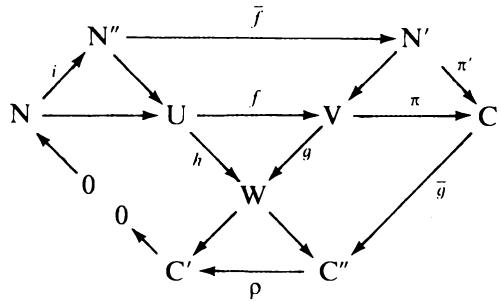
\includegraphics[keepaspectratio]{images/part002_9769358f.jpg}}\\
图 1

根据假设，N、N'、C 和 C' 都是有限维的；因此 N'' 和 C'' 也是如此。由推论 2（II，第 295 页）我们于是有

\[
[ \mathrm{N}: \mathrm{L} ] - [ \mathrm{N} ^ {\prime \prime}: \mathrm{L} ] + [ \mathrm{N} ^ {\prime}: \mathrm{L} ] - [ \mathrm{C}: \mathrm{L} ] + [ \mathrm{C} ^ {\prime \prime}: \mathrm{L} ] - [ \mathrm{C} ^ {\prime}: \mathrm{L} ] = 0
\]

由此 \(\chi(h) = \chi(f) + \chi(g)\) 。

\subsection{有限生成扩张的微分性质}

定理 4. --- 设 P 为完全域，L 为 P 的扩域，K 为 L 的子扩张；我们假设 L 是 K 的有限生成扩张。则典范 L-线性映射 \(\alpha: \Omega_{\mathrm{P}}(\mathrm{K}) \otimes_{\mathrm{K}} \mathrm{L} \to \Omega_{\mathrm{P}}(\mathrm{L})\) 的指标等于 L 在 K 上的超越次数。

如果 E 和 F 是 L 的两个子扩张，使得 \(E \subset F\) ，我们用 \(\alpha(F/E)\) 表示 \(\Omega_{\mathrm{P}}(\mathrm{E}) \otimes_{\mathrm{E}} F\) 到 \(\Omega_{\mathrm{P}}(\mathrm{F})\) 中的典范 F-线性映射，当它有定义时， \(\alpha(F/E)\) 的指标将记作 \(d(F/E)\) 。如果 E、F 和 G 是 L 的三个子扩张，使得 \(E \subset F \subset G\) ，我们有一个交换图

\[
\begin{array}{c} \Omega_ {\mathrm{P}} (\mathrm{F}) \otimes_ {\mathrm{F}} \mathrm{G} \xrightarrow {\alpha (\mathrm{G} / \mathrm{F})} \Omega_ {\mathrm{P}} (\mathrm{G}) \\ \alpha (\mathrm{F} / \mathrm{E}) \otimes_ {\mathrm{F}} \mathrm{Id} _ {\mathrm{G}} \Bigg | _ {\uparrow} \\ (\Omega_ {\mathrm{P}} (\mathrm{E}) \otimes_ {\mathrm{E}} \mathrm{F}) \otimes_ {\mathrm{F}} \mathrm{G} \xrightarrow {\beta} \Omega_ {\mathrm{P}} (\mathrm{E}) \otimes_ {\mathrm{E}} \mathrm{G} \end{array}
\]

其中 \(\beta\) 是命题 2（II，第 278 页）中定义的典范同构。由于指标在标量扩张下显然不变，且同构的指标为零，引理 2（V，第 133 页）表明指标 \(d(\mathrm{G}/\mathrm{E})\) 在 \(d(\mathrm{F}/\mathrm{E})\) 与 \(d(\mathrm{G}/\mathrm{F})\) 皆有定义时有定义，并且此时

\[
d (\mathrm{G} / \mathrm{E}) = d (\mathrm{G} / \mathrm{F}) + d (\mathrm{F} / \mathrm{E}).\tag{5}
\]

由于 L 是 K 的有限生成扩张，公式 (5) 和 V，第 111 页的推论表明，只需考虑存在 x 使得 \(L = K(x)\) 的情形；进一步地，若 x 在 K 上是代数的，则存在 L 的特征指数的某个幂 q，使得 \(x^{q}\) 在 K 上是可分代数的（V，第 44 页，命题 13）。因此，只需在以下三种特殊情形下建立等式 \(d(\mathrm{L}/\mathrm{K}) = \operatorname{tr} \cdot \deg_{\mathrm{K}} \mathrm{L}\) ：

\begin{enumerate}
\def\labelenumi{\alph{enumi})}
\item
  \(x\) 在 \(\mathbf{K}\) 上是超越的：则 \(\alpha\) 是单射且其余核在 \(\mathrm{L}(\mathrm{V},\mathrm{p}.129,\mathrm{Cor.})\) 上的秩为 1；所以我们有 \(d(\mathrm{L} / \mathrm{K}) = 1\) 并且 tr. \(\deg_{\mathbf{K}}\mathrm{L} = 1\) 。
\item
  \(x\) 在 \(\mathbf{K}\) 上是可分代数的：则 \(\alpha\) 是双射（V，第 130 页，推论 2），从而 \(d(L / K) = 0\) ；显然也有 tr. \(\deg_{\mathbf{K}}\mathbf{L} = 0\) 。
\item
  域 L 的特征为 \(p \neq 0\) , \(x \notin K\) 且 \(x^{p} = a\) 属于 K： \(\alpha\) 的余核 C 同构于 \(\Omega_{\mathrm{K}}(\mathrm{L})\) ，且由于 \(\{x\}\) 是 L 在 K 上的 p-基，空间 C 在 L 上的维数为 1（V，第 102 页，定理 1）。由于 a 是 L 中的 p 次幂，我们有 \(d_{L/P}a = 0\) 且 \(\alpha\) 的核包含 \(U = \Omega_{\mathrm{P}}(\mathrm{K}) \otimes_{\mathrm{K}} L\) 的由 \(d_{K/P}a \otimes 1\) 生成的子空间 R。对于每个 \(y \in K\) ，令 \(\Delta(y)\) 为 \(d_{K/P}y \otimes 1 \mod R\) 的剩余类；则 \(\Delta\) 是 K 到 U/R 中的一个 P-导子，使得 \(\Delta(a) = 0\) 。命题 5（V，第 101 页）表明 \(\Delta\) 可延拓为 L 到 U/R 中的一个 P-导子 D。因此存在一个 L-线性映射 \(\beta : \Omega_{\mathrm{P}}(\mathrm{L}) \to \mathrm{U}/\mathrm{R}\) 使得 \(D = \beta \circ d_{L/P}\) 且 \(\beta \circ \alpha\) 是 U 到 U/R 上的典范映射。这就证明了 R 是 \(\alpha\) 的核。由于 P 是完全域，我们有 \(P(K^{p}) = K^{p}\) ，从而 \(a \notin P(K^{p})\) ，最终 \(d_{K/P}a \neq 0\) （V，第 103 页，命题 6）。于是 \(\alpha\) 的核与余核的维数均为 1，从而 \(d(\mathrm{L}/\mathrm{K}) = 0\) ，并且我们也有 tr. deg \(_{K}L = 0\) 。
\end{enumerate}

推论 1. --- 设 L 是域 K 的有限生成扩张，其超越次数为 s。向量空间 \(\Omega_{\mathrm{K}}(\mathrm{L})\) 在 L 上的维数为 \(\geqslant s\) ，当且仅当 L 在 K 上可分时取等号。

设 P 为 K 的素子域。设 N 为 \(\alpha\) 的核，则由序列 \((\mathrm{E}_{\mathrm{P},\mathrm{K},\mathrm{L}})(\mathrm{V},\mathrm{p}.128)\) 的正合性及定理 4，我们有 \([\Omega_{\mathrm{K}}(\mathrm{L}):\mathrm{L}] = s + [\mathrm{N}:\mathrm{L}]\) ；由 V，第 132 页，推论，K 的扩张 L 是可分的当且仅当 N = 0。推论随之成立。

推论 2. --- 设 L 是域 K 的有限生成扩张。要使 L 在 K 上是代数的且可分的，其充分必要条件为 \(\Omega_{\mathbf{K}}(\mathbf{L}) = 0\) 。

这直接由推论 1 得出。

推论 3. --- 设 K 是一个特征为 \(p \neq 0\) 的域，L 是 K 的超越次数为 s 的有限生成扩张。若 \([K:K^{p}]\) 是有限的，则 \([L:L^{p}]\) 亦然，并且我们有 \([L:L^{p}] = p^{s} \cdot [K:K^{p}]\) 。

设 P 为 K 的素子域。若 \([K:K^{p}]\) 是有限的，则向量空间 \(\Omega_{\mathrm{P}}(\mathrm{K})=\Omega_{\mathrm{K}^{\mathrm{p}}}\left(\mathrm{K}\right)\) 在 K 上具有有限维数 m，并且我们有 \([K:K^{p}]=p^{m}(V,p.103,Th.2)\) ；于是向量空间 \(\Omega_{\mathrm{P}}(\mathrm{K})\otimes_{\mathrm{K}}L\) 在 L 上的维数也是有限的 m。进一步，由于 K 在 \(K^{p}\) 上的次数有限，域 \(\mathrm{K}(L^{p})\) 在 \(\mathrm{K}^{p}(L^{p})=L^{p}\) 上是有限次的；由于域 L 是 K 的有限生成扩张且在 \(\mathrm{K}(L^{p})\) 上是代数的，它是 \(\mathrm{K}(L^{p})(\mathrm{V},p.18,Th.2)\) 的有限次扩张；于是我们得出结论，L 在 \(L^{p}(V,p.10,Th.1)\) 上是有限次的。于是 \(\Omega_{\mathrm{P}}(\mathrm{L})\) 是 L 上有限维数为 n 的向量空间，并且我们有 \([L:L^{p}]=p^{n}(V,p.103,Th.2)\) 。根据引理 1（V，第 132 页），L-线性映射 \(\alpha:\Omega_{\mathrm{P}}(\mathrm{K})\otimes_{\mathrm{K}}L\to\Omega_{\mathrm{P}}(\mathrm{L})\) 因此具有指标 n-m，由此根据定理 4（V，第 133 页）得 n-m=s，且 \(p^{n}=p^{s}\cdot p^{m}\) 。

注记. --- 1) 设 K 为一个特征为 \(p \neq 0\) 的域，L 是 K 的一个扩域。我们有 \(\Omega_{\mathbf{K}}(\mathbf{L}) = 0\) 当且仅当 \(\mathbf{L} = \mathbf{K}(\mathbf{L}^p)\) （V，第 103 页，命题 6）。因此，若 L 在 K 上有限生成，则 L 是 K 上的代数可分扩张当且仅当我们有 \(\mathbf{L} = \mathbf{K}(\mathbf{L}^p)\) 。当 L 不是在 K 上有限生成时，此结果一般不再成立，正如 L 是 K 的完全闭包的情形所示。

\begin{enumerate}
\def\labelenumi{\arabic{enumi})}
\setcounter{enumi}{1}
\tightlist
\item
  设 K 为一个域， \(F_{1}, \ldots, F_{m}\) 为 \(K[X_{1}, \ldots, X_{n}]\) 中的多项式，且 L 是由元素 \(x_{1}, \ldots, x_{n}\) 生成的 K 的扩域。假设多项式 \(F_{1}, \ldots, F_{m}\) 生成 \(K[X_{1}, \ldots, X_{n}]\) 中由所有满足 \(F(x_{1}, \ldots, x_{n}) = 0\) 的多项式 F 组成的理想。由命题 1（V，第 127 页）和微分模的泛性质（III，第 569 页），我们容易推出以下结果：向量空间 \(\Omega_{K}(L)\) （在 L 上的）由 \(dx_{1}, \ldots, dx_{n}\) 生成；我们有关系
\end{enumerate}

\[
\sum_ {i = 1} ^ {n} \mathrm{D} _ {i} \mathrm{F} _ {j} (x _ {1}, \dots , x _ {n}) \cdot d x _ {i} = 0 \quad (\text { for } 1 \leqslant j \leqslant m);\tag{6}
\]

最后，如果 \(u_1, \ldots, u_n\) 是 \(L\) 的元素，使得 \(\sum_{i=1}^{n} u_i \cdot dx_i = 0\) ，则存在元素 \(v_1, \ldots, v_m\) （\(L\) 的），使得 \(u_i = \sum_{j=1}^{m} D_i F_j(x_1, \ldots, x_n) v_j\) （对于 \(1 \leqslant i \leqslant n\) ）。令 \(r\) 为矩阵 \((D_i F_j(x_1, \ldots, x_n))\) （具有 \(n\) 行和 \(m\) 列）的秩；令 \(s\) 为 L 在 K 上的超越次数。那么我们有 \([\Omega_{\mathrm{K}}(\mathrm{L}):\mathrm{L}]=n-r\) 。因此，K 的扩域 L 是可分的当且仅当 \(r+s=n\) （推论 1），并且它是代数且可分的当且仅当 r=n（推论 2）。

\subsection{可分超越基}

定义 1. --- 设 L 是域 K 的一个扩张。L 在 K 上的一个超越基 B 被称为可分的，如果 L 作为 K(B) 的代数扩张是可分的。

若 K 的特征为 0，则 L 在 K 上的每个超越基都是可分的，因为特征为 0 的域的每个代数扩张都是可分的（V，第 37 页，推论）。若一个扩张具有可分超越基，则它是可分的（V，第 121 页，命题 6 及第 122 页，命题 9）。下面的定理表明，每个有限生成的可分扩张都具有可分超越基；这一限制是本质的（V，第 177 页，习题 1）。

定理 5. --- 设 K 是一个域，L 是 K 的一个扩域，且 \((x_{i})_{i\in I}\) 是 L 的一个元素族。若该族 \((x_{i})_{i\in I}\) 是 L 在 K 上的一个可分超越基，则族 \((dx_{i})_{i\in I}\) 是向量空间 \(\Omega_{\mathrm{K}}(\mathrm{L})\) 在 L 上的一组基。若 L 是 K 的有限生成可分扩张，则逆命题成立。

令 \(\mathbf{M} = \mathbf{K}(x_i)_{i \in I}\) ，并用 \(\alpha\) 表示 \(\Omega_{\mathbf{K}}(\mathbf{M}) \otimes_{\mathbf{M}} \mathbf{L}\) 到 \(\Omega_{\mathbf{K}}(\mathbf{L})\) 中的典范映射。若 \((x_i)_{i \in I}\) 是 L 在 K 上的可分超越基，则族 \((d_{\mathbf{M}/\mathbf{K}} x_i)_{i \in I}\) 是向量 M-空间 \(\Omega_{\mathbf{K}}(\mathbf{M})\) 的一组基（V，第 128 页，命题 3），且 \(\alpha\) 是向量 L-空间的一个同构，因为 L 在 M 上是代数且可分的（V，第 130 页，推论 2）。由于 \(\alpha(d_{\mathbf{M}/\mathbf{K}} x_i \otimes 1) = d_{\mathbf{L}/\mathbf{K}} x_i\) ，族 \((d_{\mathbf{L}/\mathbf{K}} x_i)_{i \in I}\) 因此是 \(\Omega_{\mathbf{K}}(\mathbf{L})\) 在 L 上的一组基。

反之，假设 L 是 K 的一个可分有限生成扩张，并且族 \((d_{L/K}x_{i})_{i\in I}\) 是向量空间 \(\Omega_{K}(L)\) 在 L 上的一组基。由 V，第 134 页的推论 1，L 在 K 上的超越次数等于 \(\Omega_{K}(L)\) 在 L 上的维数，因此等于 I 的基数。由正合序列 \((\mathrm{E}_{\mathrm{K},\mathrm{M},\mathrm{L}})(\mathrm{V},\mathrm{p}.128)\) 我们有 \(\Omega_{\mathrm{M}}(\mathrm{L})=0\) ；由于 L 是 M 的有限生成扩张，V 第 135 页推论 2 表明 L 在 \(\mathbf{M}=\mathbf{K}(x_{i})_{i\in I}\) 上是代数且可分的；由于 L 在 K 上的超越次数是有限的且等于 I 的基数，族 \((x_{i})_{i\in I}\) 是 L 在 K 上的一个超越基（V，第 110 页，推论 1）。

推论. --- 设 L 是 K 的一个可分有限生成扩张，并设 S 是 L 的一个子集，使得 \(L = K(S)\) 。则存在 L 在 K 上的一个可分超越基 B，包含于 S 中。

由于 \(\Omega_{\mathrm{K}}(\mathrm{L})\) 由 S 中元素的微分生成，存在 S 的 s 个元素 \(x_{1}, \ldots, x_{s}\) ，使得 \((dx_{1}, \ldots, dx_{s})\) 是 \(\Omega_{\mathrm{K}}(\mathrm{L})\) 在 L 上的一组基。现在只需应用定理 5。

注记. --- 设 L 是特征为 \(p \neq 0\) 的域 K 的一个可分有限生成扩张；可能存在 L 的并非可分的超越基。只需观察到 \(\{X^{p}\}\) 是 \(\mathrm{K}(\mathbf{X})\) 的一个超越基，但 \(\mathrm{K}(\mathbf{X})\) 是 \(\mathrm{K}(\mathbf{X}^{p})\) 的次数为 p 的 p-根式扩张。

命题 5. --- 设 L 和 M 是域 K 的两个扩张，包含于一个给定的扩张中，且在 K 上代数不相交。若 M 在 K 上可分，则 L(M) 在 L 上可分。

只需证明对于 M 的每个有限子集 S，L(S) 在 L 上可分即可（V，第 122 页，命题 8）。设 S 为 M 的有限子集。由于域 K(S) 在 K 上可分，故其具有可分超越基 B（定理 5 的推论）。由于 L 与 M 在 K 上代数不相交，B 是 L(B) 在 L 上的超越基（V，第 113 页，命题 12）。进一步，S 的每个元素在 K(B) 上都是代数且可分的，因此在 L(B) 上亦然（V，第 39 页，推论 2）。我们由此推出（V，第 39 页，命题 6）L(S) = L(B)(S) 在 L(B) 上是代数且可分的，因此 L(S) 在 L 上可分。

推论. --- 若 L 与 M 是 K 上可分且代数不相交的扩张，则域 \(\mathbf{K}(\mathbf{L} \cup \mathbf{M})\) 在 K 上是可分的。

由于 \(K(L \cup M) = L(M)\) 由命题 5 在 L 上是可分的（因为 M 在 K 上是可分的），且 L 在 K 上是可分的，故得推论（V，第 122 页，命题 9）。

\pandocbounded{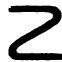
\includegraphics[keepaspectratio]{images/part002_2c83366d.jpg}}

L 和 M 的扩张在代数上不相交这一假设在命题 5 及其推论中是必不可少的。因为设 K 是一个特征为 \(p \neq 0\) 的非完全域，E 是形如 \(\mathrm{K}(x, a)\) 的扩张，其中 x 在 K 上超越，a 是 K 上高度为 1 的 p-根式元；令 \(\mathrm{L} = \mathrm{K}(x)\) 且 \(\mathrm{M} = \mathrm{K}(x + a)\) 。则 \(x + a\) 在 K 上超越（若非如此， \(x = (x + a) - a\) 将在 K 上代数），且域 L 与 M 在 K 上可分。然而， \(\mathrm{K}(\mathrm{L} \cup \mathrm{M}) = \mathrm{K}(x, a)\) 是 \(\mathrm{L} = \mathrm{K}(x)\) 上的次数为 p 的 p-根式扩张，且在 L 上不可分，在 K 上也不可分。

\section{正则扩张}

\subsection{关于相对可分代数闭包的补充}

定理 1（Zariski）。--- 设 K 是一个域，L 是 K 的一个扩域， \(K_{1}\) 是 K 在 L 中的相对可分代数闭包（V，第 44 页）， \(K_{2}\) 是 K 在 L 中的相对代数闭包（V，第 19 页），以及 \((\mathbf{X}_{i})_{i\in I}\) 是一组未定元。那么 \(\mathrm{K}_{1}(\mathbf{X}_{i})_{i\in I}\) 是 \(\mathrm{K}(\mathbf{X}_{i})_{i\in I}\) 在 \(\mathrm{L}(\mathbf{X}_{i})_{i\in I}\) 中的相对可分代数闭包，且 \(\mathrm{K}_{2}(\mathbf{X}_{i})_{i\in I}\) 是 \(\mathrm{K}(\mathbf{X}_{i})_{i\in I}\) 在 \(\mathrm{L}(\mathbf{X}_{i})_{i\in I}\) 中的相对代数闭包。

\begin{enumerate}
\def\labelenumi{\Alph{enumi})}
\tightlist
\item
  设 E 是一个域，F 是 E 的一个扩域，并且 F 中每个在 E 上可分代数的元素都属于 E。令 u 为 \(F(X)\) 中的一个在 \(E(X)\) 上可分代数的元素；我们将证明 u 属于 \(E(X)\) 。在 \(F(X)\) 中存在两个互素的多项式 P 和 Q，使得 u = P/Q，并且我们可以取 Q 为首一多项式。设 S 为 F 的由 P 和 Q 的系数组成的有限子集， \(F_{0} = E(S)\) ，并令 \(\Delta\) 为 \(\mathbf{F}_0\) 到 \(\mathbf{F}_0\) 中的一个 E-导子。设 \(D\) 为 \(\mathrm{F}_0(\mathbf{X})\) 到自身的、与 \(\Delta\) 在 \(\mathbf{F}_0\) 上一致且把 \(X\) 映为 0 的导子（V，第 128 页，命题 3）。
\end{enumerate}

由于 \(u \in F_0(X)\) 在 \(E(X)\) 上是可分代数的，且 \(D\) 在 \(E(X)\) 上为零，我们有 \(D(u) = 0\) （V，第 129 页，命题 4），由此 \(D(P).Q = P.D(Q)\) 。由于 \(P\) 和 \(Q\) 是互素的，我们得出结论 \(Q\) 整除 \(D(Q)\) （IV，第 13 页，推论 4）。现在 \(Q\) 可以写成形式

\[
\mathrm{Q} (\mathrm{X}) = \mathrm{X} ^ {n} + a _ {1} \mathrm{X} ^ {n - 1} + \dots + a _ {n - 1} \mathrm{X} + a _ {n}
\]

其中 \(a_1, \ldots, a_n\) 属于 \(\mathbf{F}_0\) ；由于 \(\mathbf{D}(x) = 0\) ，因此我们有

\[
\mathrm{D} (\mathrm{Q}) = \Delta (a _ {1}) \mathrm{X} ^ {n - 1} + \dots + \Delta (a _ {n - 1}) \mathrm{X} + \Delta (a _ {n})\tag{1}
\]

由此 \(\deg D(Q) < \deg Q\) 。由于 \(Q\) 整除 \(D(Q)\) ，这只有在 \(D(Q) = 0\) 时才可能。但此时 \(D(P) = 0\) ，因为 \(D(P) \cdot Q = P \cdot D(Q)\) 。现在 (1) 以及对于 \(P\) 的一个类似公式表明 \(\Delta\) 零化系数集合 \(S\) （\(P\) 和 \(Q\) 的），从而 \(\Delta = 0\) ，因为 \(F_0 = E(S)\) 。根据 \(V\) ，第 135 页，推论 2，有限生成扩张 \(F_0\) （\(E\) 的）因此是可分代数的；根据关于 \(E\) 和 \(F\) 的假设我们有 \(F_0 = E\) ，所以最终 \(u \in E(X)\) 。

\begin{enumerate}
\def\labelenumi{\Alph{enumi})}
\setcounter{enumi}{1}
\item
  现在假设 E 在扩域 F 中是相对代数封闭的，并记 p 为 E 的特征指数。设 u 是 \(F(X)\) 中的一个在 \(E(X)\) 上代数的元素。存在一个整数 \(f \geqslant 0\) 使得 \(v = u^{p^f}\) 在 \(E(X)\) 上是可分代数的（V，第 44 页，命题 13）。由 A) 我们因此有 \(v \in E(X)\) 。存在 u 的形如 P/Q 的唯一表示，其中 P 和 Q 是 F{[}X{]} 中互素的多项式且 Q 为首一的；我们有类似的分解 \(v = P_1 / Q_1\) ，其中 \(P_1\) 和 \(Q_1\) 在 E{[}X{]} 中互素，且 \(Q_1\) 是首一的。由此可知 \(P_1 / Q_1 = P^{p^f} / Q^{p^f}\) ；多项式 \(P^{p^f}\) 和 \(Q^{p^f}\) 在 F{[}X{]} 中互素（IV，第 13 页，推论 6），如同 \(P_1\) 和 \(Q_1\) 一样，且 \(Q^{p^f}\) 是首一的。由此可得 \(P^{p^f} = P_1 \in E[X]\) 且 \(Q^{p^f} = Q_1 \in E[X]\) 。因此 P 和 Q 的系数在 E 上是 p-根式的，从而属于 E，因为 E 在 F 中是相对代数封闭的。我们因此有 \(P \in E[X]\) , \(Q \in E[X]\) 并且最终 \(u \in E(X)\) 。这证明了 \(E(X)\) 在 F(X) 中是相对代数封闭的。
\item
  我们使用定理 1 的记号。由于 \(\mathbf{K}_1\) 是 \(\mathbf{K}\) 的一个可分代数扩张，扩张 \(\mathbf{K}_1(\mathbf{X}_i)_{i\in I}\) （\(\mathbf{K}(\mathbf{X}_i)_{i\in I}\) 的扩张）是代数的且可分的（V，第 39 页，命题 6）。此外， \(L\) 的每个在 \(\mathbf{K}_1\) 上代数且可分的元素都属于 \(\mathbf{K}_1\) （V，第 44 页，命题 13, a)）。设 \(J\) 是 \(I\) 的一个有限子集；通过对 \(J\) 的基数的直接归纳，我们由 \(A\) ) 推出， \(\mathrm{L}(\mathbf{X}_i)_{i\in J}\) 的每个在 \(\mathbf{K}(\mathbf{X}_i)_{i\in J}\) 上代数且可分的元素都属于 \(\mathbf{K}_1(\mathbf{X}_i)_{i\in J}\) 。最后设 \(u\) 是 \(\mathrm{L}(\mathbf{X}_i)_{i\in I}\) 的一个在 \(\mathbf{K}(\mathbf{X}_i)_{i\in I}\) 上代数且可分的元素；存在一个有限子集 \(J\) （\(I\) 的），使得 \(u\) 属于 \(\mathrm{L}(\mathbf{X}_i)_{i\in J}\) 且在 \(\mathbf{K}(\mathbf{X}_i)_{i\in J}\) 上是代数且可分的；根据前述内容， \(u\) 属于 \(\mathbf{K}_1(\mathbf{X}_i)_{i\in J}\) ，更不用说属于 \(\mathbf{K}_1(\mathbf{X}_i)_{i\in I}\) 了。
\end{enumerate}

我们由此从 \(A\) 推出 \(\mathrm{K}_1(\mathbf{X}_i)_{i\in I}\) 是 \(\mathrm{K}(\mathbf{X}_i)_{i\in I}\) 在 \(\mathrm{L}(\mathbf{X}_i)_{i\in I}\) 中的相对可分闭包；同样地，由 \(B\) 推出 \(\mathrm{K}_2(\mathbf{X}_i)_{i\in I}\) 是 \(\mathrm{K}(\mathbf{X}_i)_{i\in I}\) 在 \(\mathrm{L}(\mathbf{X}_i)_{i\in I}\) 中的相对代数闭包。

\subsection{扩张的张量积}

命题 1. --- 设 \(\Omega\) 是域 \(K\) 的一个扩张，并令 \(L, M\) 为 \(\Omega\) 的两个在 \(K\) 上代数不相交的子扩张。假设 \(K\) 在 \(L\) 中的相对可分代数闭包等于 \(K^1\) 。设 \(\varphi\) 为 \(L \otimes_K M\) 到 \(\Omega\) 中的 K-代数同态，它把 \(x \otimes y\) 映为 \(xy\) （对于 \(x \in L\) , \(y \in M\) ），并设 \(\mathfrak{p}\) 是 \(\varphi\) 的核，则 \(\mathfrak{p}\) 是 \(L \otimes_K M\) 的幂零元集合，且它是 \(L \otimes_K M\) 的最小素理想。

必要时将 \(\Omega\) 替换为一个代数闭包，我们可以假设 \(\Omega\) 是代数闭的。设 B 为 M 在 K 上的一个超越基，N 为 \(\mathrm{K}(\mathrm{B})\) 在 \(\Omega\) 中的相对代数闭包， \(\mathrm{N}_{s}\) （相应地 \(N_{r}\) ）为 N 的在 \(\mathrm{K}(\mathrm{B})\) 上可分（相应地，p-根式）的元素集合。我们注意到 M 在 \(\mathrm{K}(\mathrm{B})\) 上是代数的，因此 N 是 M 在 \(\Omega\) 中的相对代数闭包。

\pandocbounded{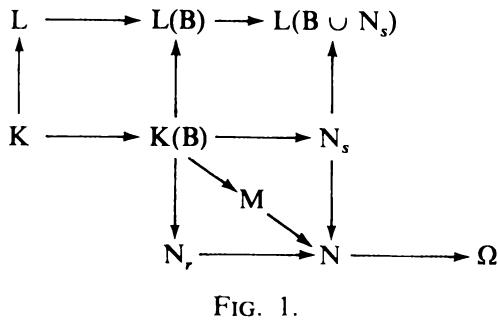
\includegraphics[keepaspectratio]{images/part002_5eeda79f.jpg}}

让我们定义以下同态链：

\[
\begin{array}{r l} & {\mathrm{L} \otimes_ {\mathrm{K}} \mathrm{M} \xrightarrow {\alpha} \mathrm{L} \otimes_ {\mathrm{K}} \mathrm{N} \xrightarrow {\beta} (\mathrm{L} \otimes_ {\mathrm{K}} \mathrm{K} (\mathrm{B})) \otimes_ {\mathrm{K} (\mathrm{B})} \mathrm{N} \xrightarrow {\gamma} \mathrm{L} (\mathrm{B}) \otimes_ {\mathrm{K} (\mathrm{B})} \mathrm{N}} \\ & {\xrightarrow {\delta} \mathrm{L} (\mathrm{B}) \otimes_ {\mathrm{K} (\mathrm{B})} \mathrm{N}_s \otimes_ {\mathrm{K} (\mathrm{B})} \mathrm{N}_r \xrightarrow {\varepsilon} \mathrm{L} (\mathrm{B} \cup \mathrm{N}_s) \otimes_ {\mathrm{K} (\mathrm{B})} \mathrm{N}_r \xrightarrow {\zeta} \Omega .} \end{array}
\]

我们有 \(\alpha = \mathrm{Id}_{\mathbf{L}} \otimes u\) ，其中 \(u\) 是 M 到 N 中的典范嵌入，因此 \(\alpha\) 是单射。映射 \(\beta\) 是交换群的同构，它把 \(x \otimes y\) 映为 \((x \otimes 1) \otimes y\) （II，第 278 页，命题 2），对于 \(x \in L\) 和 \(y \in N\) 。我们有 \(\gamma = v \otimes \mathrm{Id}_{\mathbf{N}}\) ，其中 \(v\) 是 \(\mathrm{L} \otimes_{\mathbf{K}} \mathrm{K}(\mathrm{B})\) 到 \(\mathrm{L}(\mathrm{B})\) 中的、把 \(x \otimes y\) 映为 \(xy\) 的 K-代数同态（对于 \(x \in L\) 和 \(y \in \mathrm{K}(\mathrm{B})\) ）；由于 L 和 M 在 K 上代数不相交，命题 14（V，第 114 页）表明 L 和 K(B) 在 K 上线性不相交，换言之， \(v\) 是单射，因此 \(\gamma\) 是单射。由于 N 是 K(B) 的拟伽罗瓦扩张，存在（V，第 76 页，命题 13）一个 K(B)-代数同构 \(w\) ，它把 \(\mathrm{N}_s \otimes_{\mathrm{K}(\mathrm{B})} \mathrm{N}_r\) 同构地映到 N 上，并把 \(x \otimes y\) 映为 \(xy\) （对于 \(x \in \mathbf{N}_s\) 和 \(y \in \mathbf{N}_r\) ）；我们用 \(\delta\) 表示同构 \(\mathrm{Id}_{\mathrm{L(B)}} \otimes w^{-1}\) 。由定理 1（V，第 137 页）以及关于 K 的扩张 L 的假设，L(B) 中每个在 K(B) 上代数且可分的元素都属于 K(B)；特别地，我们有 L(B) \(\cap\) N \(_s\) = K(B)。由于 N \(_s\) 是 K(B) 的伽罗瓦扩张，定理 5（V，第 71 页）表明存在一个 K(B)-代数同构 \(w'\) ，它是 L(B) \(\otimes_{\mathrm{K(B)}} \mathrm{N}_s\) 到 L(B \(\cup\) N \(_s\) ) 上的、把 \(x \otimes y\) 映为 \(xy\) 的映射（对于 \(x \in L(B)\) 和 \(y \in \mathrm{N}_s\) ）；我们用 \(\varepsilon\) 表示同构 \(w' \otimes \mathrm{Id}_{\mathrm{N}_r}\) 。最后， \(\zeta\) 是把 \(x \otimes y\) 映为 \(xy\) 的 K-代数同态（对于 \(x \in L(B \cup \mathrm{N}_s)\) 和 \(y \in \mathrm{N}_r\) ）。

以上所述表明， \(\eta = \varepsilon \delta \gamma \beta \alpha\) 是 \(L \otimes_{K} M\) 到 \(L(B \cup N_s) \otimes_{K(B)} N_r\) 中的单 K-代数同态。进一步地， \(M\) 的每个元素具有形式 \(\sum_{i=1}^{n} a_i b_i\) ，其中 \(a_i \in N_s\) 且 \(b_i \in N_r\) （对于 \(1 \leqslant i \leqslant n\) ）；因此我们得到 \(\varphi = \zeta \eta\) 。

核 \(\mathfrak{p}\) （\(\varphi\) 的）是 \(\mathbf{L} \otimes_{\mathbb{K}} \mathbf{M}\) 的一个素理想，因此由命题 2（V，第 118 页）， \(\mathbf{L} \otimes_{\mathbb{K}} \mathbf{M}\) 的每个幂零元素都属于 \(\mathfrak{p}\) 。反之设 \(a\) 为 \(\mathfrak{p}\) 的一个元素；令 \(\eta(a) = \sum_{i=1}^{s} b_i \otimes c_i\) ，其中 \(b_i \in \mathbf{L}(\mathbf{B} \cup \mathbf{N}_s)\) 且 \(c_i \in \mathbf{N}_r\) （对于 \(1 \leqslant i \leqslant s\) ）。由于

\(N_{r}\) 是 \(K(B)\) 的一个 p-根式扩张，存在一个整数 \(f \geqslant 0\) 使得 \(c_{i}^{p^{f}}\) 属于 \(K(B)\) （对于 \(1 \leqslant i \leqslant s\) ，其中 p 是 K 的特征指数）。但我们有

\[
\eta \left(a ^ {p ^ {f}}\right) = \sum_ {i = 1} ^ {s} b _ {i} ^ {p ^ {f}} \otimes c _ {i} ^ {p ^ {f}} = \left(\sum_ {i = 1} ^ {s} b _ {i} ^ {p ^ {f}} c _ {i} ^ {p ^ {f}}\right) \otimes 1 = \zeta \eta (a) ^ {p ^ {f}} \otimes 1 = 0
\]

且由于 \(\eta\) 是单射，我们最终有 \(a^{p^{f}} = 0\) 。因此我们已证明 \(\mathfrak{p}\) 是 \(\mathrm{L} \otimes_{\mathrm{K}} \mathrm{M}\) 的所有幂零元素的集合。现在，由命题 2（V，第 118 页）， \(\mathrm{L} \otimes_{\mathrm{K}} \mathrm{M}\) 的每个素理想都包含 \(\mathfrak{p}\) 。

推论. --- 设 L 和 M 是域 K 的两个扩域。假设 K 在 L 中的相对可分代数闭包等于 K。则 \(L \otimes_{K} M\) 的幂零元集合 p 是一个素理想。此外，如果 L 或 M 在 K 上是可分的，则 \(L \otimes_{K} M\) 是整环。

我们可以假设 L 和 M 是 K 的某个扩张 \(\Omega\) 的代数不相交的子扩张（V，第 116 页，定理 5）；则根据命题 1（V，第 139 页），p 是素理想。若进一步 L 或 M 在 K 上可分，则由可分扩张的定义（V，第 119 页，定义 1）， \(L \otimes_{K} M\) 是既约环；所以 p = 0 且 \(L \otimes_{K} M\) 是整环，因为 p 原先是素理想。

\subsection{正则代数}

定义 1. --- 设 K 为一个域。称 K 上的代数 A 是正则的，如果对于 K 的每一个扩域 L，L ⊗K A 都是整环。

正则代数尤其是一个整环，因此是交换的。

命题 2. --- 设 A 和 B 是域 K 上的两个代数。若 A 是整环且 B 是正则的，则 \(A \otimes_{K} B\) 是整环。

设 \(L\) 为 \(A\) 的分式域。由于 \(B\) 是一个正则 \(K\) -代数， \(L \otimes_K B\) 是整环，因此 \(A \otimes_K B\) 亦然，因为它同构于 \(L \otimes_K B\) 的一个子环。

命题 3. --- 设 K 是一个域。

\begin{enumerate}
\def\labelenumi{\alph{enumi})}
\item
  正则 K-代数的每个子代数本身都是正则的。
\item
  两个正则 K-代数的张量积仍然是正则的。
\item
  设 A 是一个 K-代数，且 \(K'\) 是 K 的一个扩张。要使 A 为正则，必要且充分条件是由 A 通过标量扩张得到的 \(K'\) -代数 \(\mathrm{A}_{(\mathbb{K}')}\) 是正则的。
\end{enumerate}

\(a\) （相应地 \(c\) ) 的证明与 V，第 119 页命题 3 的部分 \(a\) （相应地 \(d\) ) 的证明相同，只需在处处将“既约环”替换为“整环”、“可分代数”替换为“正则代数”。我们来证明 \(b\) ).

设 A 和 B 是两个正则 K-代数。设 L 是 K 的一个扩张。由于 A 是正则的，环 \(L \otimes_{K} A\) 是整环。根据命题 2，环 \((L \otimes_{K} A) \otimes_{K} B\) 是整环，因为 B 是正则的。最后，环 \(L \otimes_{K} (A \otimes_{K} B)\) 同构于 \((L \otimes_{K} A) \otimes_{K} B\) ，因此是一个整环。这表明 \(A \otimes_{K} B\) 是一个正则 K-代数。

\subsection{正则扩张}

定义 2. --- 域 K 的一个扩张称为正则的，如果它作为 K-代数是正则的。

命题 4. --- 设 A 是域 K 上的一个代数，且为整环，E 是它的分式域。设 L 是 K 的一个扩张；若环 \(L \otimes_{K} A\) 是整环，则 \(L \otimes_{K} E\) 亦然。

如果 \(L \otimes_{K} A\) 是整环，则它可以嵌入到它的分式域 F 中。记 \(u(x) = x \otimes 1\) （对于 \(x \in L\) ），并用 v 表示 E 到 F 中的、延拓 A 到 F 中的单同态 \(y \mapsto 1 \otimes y\) 的 K-同态。由命题 6（V，第 14 页），F 的子域 \(u(L)\) 和 \(v(E)\) 在 K 上线性不相交；因此，\(u * v\) 作为 \(L \otimes_{K} E\) 到 F 中的同态（V，第 12 页）是单射。这表明 \(L \otimes_{K} E\) 是一个整环。

推论. --- 要使 A 是正则 K-代数，必要且充分条件是它的分式域是 K 的正则扩张。

该条件由命题 4 可知是必要的，由命题 3，a) 可知是充分的。

命题 5. --- 域 K 的每一个纯扩张都是正则的。

由前述推论，只需证明每个多项式代数 \(A = K[X_{i}]_{i \in I}\) 都是正则 K-代数。设 L 是 \(K\) 的一个扩张；环 \(L \otimes_{K} A\) 同构于 \(L[X_{i}]_{i \in I}\) （III，第 449 页，注记 2），因此是整环（IV，第 9 页，命题 8）。

命题 6. --- 设 L 是域 K 的一个扩张。若 L 是正则的，则 L 的每个子扩张都是正则的。反之，若 L 的每个有限生成子扩张都是正则的，则 L 是正则的。

第一个断言由命题 3，a) 得出。

设 M 是 K 的一个扩张，并设 U 是 L 的所有有限生成子扩张的集合。对于每个 \(E \in U\) ，环 \(M \otimes_{K} E\) 可以与 \(M \otimes_{K} L\) 的一个子环等同起来，这样我们就得到 \(M \otimes_{K} L\) 的一个递增有向子环族，其并为 \(M \otimes_{K} L\) 。于是第二个断言立即得证。

命题 7. --- 设 L 是域 K 的一个扩张，M 是一个 L-代数（例如 L 的一个扩张）。若 L 在 K 上正则且 M 是正则 L-代数，则 M 作为 K-代数是正则的。

设 E 是 K 的一个扩张；由于 L 在 K 上是正则的， \(E \otimes_{K} L\) 是整环。于是根据命题 2（V，第 141 页），环 \((\mathrm{E} \otimes_{\mathrm{K}} \mathrm{L}) \otimes_{\mathrm{L}} \mathrm{M}\) 是整环，而与它同构的环 \(E \otimes_{K} M\) （II，第 278 页，命题 2）亦然。由此即得结论。

命题 8. --- 设 L 和 M 是域 K 的两个扩张。

\begin{enumerate}
\def\labelenumi{\alph{enumi})}
\item
  如果 \(\mathbf{M}\) 在 \(\mathbf{K}\) 上是正则的，则整环 \(\mathbf{L} \otimes_{\mathbf{K}} \mathbf{M}\) 的分式域是 \(\mathbf{L}\) 的一个正则扩张。
\item
  若 L 和 M 都是 K 的正则扩张，则 L ⊗\_K M 的分式域亦然。
\end{enumerate}

断言 a) 由命题 3，c)（V，第 141 页）及 V，第 141 页的推论得出；断言 b) 由命题 3，b)（V，第 141 页）及 V，第 141 页的推论得出。

\subsection{正则扩张的刻画}

命题 9. --- 设 K 是一个域， \(\bar{K}\) 是 K 的一个代数闭包，L 是 K 的一个扩张。则下列条件等价：

\begin{enumerate}
\def\labelenumi{\alph{enumi})}
\item
  L 在 K 上是可分的，且 K 在 L 中相对代数封闭。
\item
  L 是 K 的正则扩张。
\item
  环 \(\bar{\mathbf{K}}\otimes_{\mathbb{K}}\mathbf{L}\) 是整环。
\item
  设 \(\bar{L}\) 是 L 的一个代数闭包。则 L 与 K 在 \(\bar{L}\) 中的相对代数闭包在 K 上线性不相交。
\end{enumerate}

此外，当这些条件成立时，则 \(\bar{\mathbf{K}}\otimes_{\mathbf{K}}\mathbf{L}\) 是一个域。

\(a) \Rightarrow b)\) ：设 M 是 K 的一个扩张。在 \(a\) ) 的假设下，环 M \(\otimes_{K} L\) 是整环（V，第 140 页，推论）。

\(b) \Rightarrow c)\) ：这由定义 2 得出。

\(c) \Rightarrow d): \text{记号为 } d) \text{ 我们可以识别 } \bar{\mathbf{K}} \text{ 取其相对代数闭包 } \mathbf{K} \text{ 在 } \bar{\mathbf{L}} (\mathbf{V}, \text{ p. 22, Ex. 2}). \text{ 设环 } \mathbf{A} = \bar{\mathbf{K}} \otimes_{\mathbf{K}} \mathbf{L} \text{ 是整环。令 } \mathbf{E} \text{ 为其子扩张 } \bar{\mathbf{K}} \text{ 有限次数扩张 } \mathbf{K}; \text{ 子环}\)

\(E \otimes_{K} L\) 这个 A 的子环是整环，从而是 L 上的一个有限次代数；由 V，第 10 页的推论，它是一个域。由于 \(\bar{K}\) 是上述类型的扩张 E 组成的递增有向集的并，A 是一个域（V，第 11 页，命题 3）。于是，A 到 \(\bar{L}\) 中的、把 \(x \otimes y\) 映为 xy（对于 \(x \in \bar{K}\) 和 \(y \in L\) ）的典范同态是单射，所以 L 和 \(\bar{K}\) 在 K 上线性不相交。

\(d) \Rightarrow a): \text{在其假设下 } d) \text{ 有 } L \cap \bar{K} = K, \text{ 所以 } K \text{ 在其中相对代数闭 } L; \text{ 此外，若 } p \text{ 是其特征指数 } K, \text{ 域 } L \text{ 与其线性不交 } K^{p^{-\infty}} \text{ 在其上 } K, \text{ 因此 } L \text{ 在其上可分离 } K (V, p. 123, Cor. 1).\)

推论 1. --- 设 A 是域 K 上的一个代数。要使 A 是正则 K-代数，必要且充分条件是环 \(\bar{\mathbf{K}}\otimes_{\mathbf{K}}\mathbf{A}\) 是整环。

所述条件显然是必要的。反之，假设 \(\bar{K} \otimes_{K} A\) 是一个整环，并记 E 为 A 的分式域。由命题 4（V，第 141 页），环 \(\bar{K} \otimes_{K} E\) 是一个整环，因此由命题 9，E 是 K 的正则扩张；由 V，第 141 页的推论，我们得出 A 作为 K-代数是正则的。

推论 2. --- 设 K 是一个代数闭域。每个作为整环的 K-代数都是正则 K-代数。特别地，K 的每个扩张都是正则的。

这由推论 1 得出。

推论 3. --- 设 K 是一个代数闭域。若 A 和 B 是两个作为整环的 K-代数，则 A ⊗\_K B 亦然。

根据推论 2，A 和 B 是正则 K-代数，只需应用命题 2（V，第 141 页）。

\subsection{复合扩张的应用}

命题 10. -- 设 L 和 M 是域 K 的两个扩张，(E, u, v) 是 L 和 M 的一个复合扩张（V，第 12 页）。假设环 L ⊗\_K M 是整环，且 E 的子扩张 u(L) 和 v(M) 在 K 上代数不相交。则 u(L) 和 v(M) 在 K 上线性不相交。

令 \(w = u * v\) （V，第 12 页），用 F 表示整环 \(L \otimes_{K} M\) 的分式域，并借助映射 \(x \mapsto x \otimes 1\) （相应地， \(y \mapsto 1 \otimes y\) ）把 L（相应地，M）等同于 F 的一个子域；则 w 在 L（相应地，M）上的限制是 u（相应地，v）。设 B 是 M 在 K 上的一个超越基（V，第 109 页，定理 1）。

根据假设， \(u(\mathbf{L})\) 和 \(v(\mathbf{M})\) 在 \(\mathbf{K}\) 上代数不相交；因此（V，第 114 页，命题 14）， \(u(\mathbf{L})\) 和 \(v(\mathbf{K}(\mathbf{B}))\) 在 \(\mathbf{K}\) 上线性不相交。于是存在一个 K-同态 \(u': \mathbf{L}(\mathbf{B}) \to \mathbf{E}\) ，它与 \(u\) 在 \(\mathbf{L}\) 上一致，且与 \(v\) 在 \(\mathbf{K}(\mathbf{B})\) 上一致。根据构造， \(\mathbf{L}\) 和 \(\mathbf{M}\) 在 \(\mathbf{K}\) 上于 \(\mathbf{F}\) 中线性不相交；由命题 8（V，第 15 页），子域 \(\mathbf{L}(\mathbf{B})\) 和 \(\mathbf{M}\) （\(\mathbf{F}\) 的）在 \(\mathbf{K}(\mathbf{B})\) 上线性不相交。由此可知，存在一个 K-同态 \(w' \colon \mathbf{M}[\mathrm{L}(\mathrm{B})] \to \mathrm{E}\) ，它与 \(u'\) 在 \(\mathrm{L}(\mathrm{B})\) 上一致，且与 \(v\) 在 \(\mathbf{M}\) 上一致。但域 \(F\) 由 \(\mathbf{M} \cup \mathrm{L}(\mathrm{B})\) 生成，且 \(\mathbf{M}\) 在 \(\mathbf{K}(\mathbf{B})\) 上是代数的；于是我们有 \(\mathbf{M}[\mathrm{L}(\mathbf{B})] = F(\mathbf{V}, p. 18, Cor. 2)\) 。由此我们得出结论： \(w'\) 是 \(F\) 到 \(E\) 上的一个 K-同构，它在 \(L\) （相应地， \(M\) ）上的限制是 \(u\) （相应地， \(v\) ）。这表明 \(u(L)\) 和 \(v(M)\) 在 \(K\) 上线性不相交。

推论 1. --- 设 \(\Omega\) 是域 \(K\) 的一个扩张， \(L\) 是 \(\Omega\) 的一个在 \(K\) 上正则的子扩张。每个子扩张 \(M\) （\(\Omega\) 的），只要它与 \(L\) 在 \(K\) 上代数不相交，就是线性不相交的。

由正则扩张的定义，环 \(L \otimes_{K} M\) 是一个整环，现在只需应用命题 10。

推论 2. --- 设 \(\Omega\) 是域 \(K\) 的一个扩张， \(L\) , \(M\) 是 \(\Omega\) 的两个子扩张。假设 \(L\) 在 \(K\) 上可分，且 \(K\) 在 \(M\) 中的相对可分闭包等于 \(K\) 。若 \(L\) 和 \(M\) 在 \(K\) 上代数不相交，则它们在 \(K\) 上线性不相交。

根据命题 10，只需注意到环 \(\mathbf{L} \otimes_{\mathbf{K}} \mathbf{M}\) 是整环（V，第 140 页，推论）。

\BourbakiExercises

\BourbakiExerciseGroup

\begin{enumerate}
\def\labelenumi{\arabic{enumi})}
\item
  设 A 是一个不一定交换的环，非零且无零因子（I，第 98 页）。证明：若存在整数 \(m \geqslant 1\) 使得 \(m\mathbf{A} = 0\) ，则具有此性质的所有整数组成的集合是一个理想 \(p\mathbf{Z}\) ，其中 \(p\) 是一个素数，且 A 是特征为 \(p\) 的环。
\item
  设 \(m, n\) 为满足 \(0 \leqslant n \leqslant m\) 的整数。设 \(p\) 为一个素数，并设 \(m = \alpha_0 + \alpha_1p + \cdots + \alpha_rp^r\) 与 \(n = \beta_0 + \beta_1p + \cdots + \beta_rp^r\) 为 \(m\) 和 \(n\) 在基 \(p\) 下的展开式，因而我们有 \(0 \leqslant \alpha_i < p\) ， \(0 \leqslant \beta_i < p\) （对于 \(0 \leqslant i \leqslant r\) ）；假设 \(\alpha_r \neq 0\) 。证明 \(\binom{m}{n} \equiv 0 (\bmod p)\) ，只要 \(\beta_i > \alpha_i\) 对至少一个指标 \(i\) 成立。另一方面，如果 \(\beta_i \leqslant \alpha_i\) （对于 \(0 \leqslant i \leqslant r\) ），则
\end{enumerate}

\[
\binom {m} {n} \equiv \binom {\alpha_ {0}} {\beta_ {0}} \dots \binom {\alpha_ {r}} {\beta_ {r}} \pmod {p}  .
\]

（在 \((\mathbf{Z} / p\mathbf{Z})[\mathbf{X}]\) 中，我们有 \((1 + \mathbf{X})^m = (1 + \mathbf{X})^{\alpha_0}(1 + \mathbf{X}^p)^{\alpha_1}\dots (1 + \mathbf{X}^{p^r})^{\alpha_r})\)

\begin{enumerate}
\def\labelenumi{\arabic{enumi})}
\setcounter{enumi}{2}
\tightlist
\item
  设 \(\mathbf{A}\) 为一个交换环。对于每个多项式 \(f \in \mathbf{A}[\mathbf{X}]\) ，我们在多项式环 \(\mathbf{A}[\mathbf{X}, \mathbf{Y}]\) （\(\mathbf{A}\) 上的两个未定元的多项式环）中写下
\end{enumerate}

\[
f (\mathbf {X} + \mathbf {Y}) = \sum_ {m = 0} ^ {\infty} \Delta_ {m} f (\mathbf {X}) \mathbf {Y} ^ {m},
\]

其中 \(\Delta_{m}\) 因而是 A{[}X{]} 到自身的一个 A-线性映射。\\
a) 若 Z 是一个未定元，且 \(\tau_{Z}\) 是 A{[}X{]} 到 A{[}X, Z{]} 的一个 A-线性映射，满足 \(\tau_{Z}f = f(X + Z)\) ，证明 \(\tau_{Z} \circ \Delta_{m} = \Delta_{m} \circ \tau_{Z}\) （其中右侧的 \(\Delta_{m}\) 是上面在环 B{[}X{]} 中定义的映射，其中 B = A{[}Z{]}）。由此推出，在 A{[}X{]} 中我们有

\[
\Delta_ {m} \Delta_ {n} = \Delta_ {n} \Delta_ {m} = \binom {m + n} {m} \Delta_ {m + n}
\]

对于整数 \(m, n \geqslant 0\) （参见 IV，第 8 页）。

\begin{enumerate}
\def\labelenumi{\alph{enumi})}
\setcounter{enumi}{1}
\tightlist
\item
  设 A 是特征为 p \textgreater{} 0 的环，并且对每个整数 \(k \geqslant 0\) 令 \(D_{k} = \Delta_{p^{k}}\) 。证明：若 \(f \in A[X]\) 且 \(g \in A[X^{p^{k}}]\) ，则 \(D_{k}(fg) = g \cdot D_{k}f + f \cdot D_{k}g\) 。
\end{enumerate}

每个多项式 \(f \in \mathbf{A}[\mathbf{X}]\) 都可以唯一地写成形式 \(f(\mathbf{X}) = \sum_{m=0}^{\infty} \mathbf{X}^{mp^k} g_m(\mathbf{X})\) ，其中 \(\deg(g_m) < p^k\) ；证明

\[
\mathrm{D} _ {k} f (\mathbf {X}) = \sum_ {m = 0} ^ {\infty} m \mathbf {X} ^ {(m - 1) p ^ {k}} g _ {m} (\mathbf {X})
\]

并推导出 \(D_{k}^{p}=0\)。

\begin{enumerate}
\def\labelenumi{\alph{enumi})}
\setcounter{enumi}{2}
\tightlist
\item
  对于每个整数 m \textgreater{} 0，设 \(m = \alpha_{0} + \alpha_{1}p + \cdots + \alpha_{k}p^{k}\) 为 m 在基 p 下的展开式（集合论，III，第 177 页），因而 \(0 \leqslant \alpha_{j} < p\) （对于 \(0 \leqslant j \leqslant k\) ）；假设 \(\alpha_{k} \neq 0\) 。证明
\end{enumerate}

\[
\Delta_ {m} = \left(\frac {1}{\alpha_ {0} !} D _ {0} ^ {\alpha_ {0}}\right) \left(\frac {1}{\alpha_ {1} !} D _ {1} ^ {\alpha_ {1}}\right) \dots \left(\frac {1}{\alpha_ {k} !} D _ {k} ^ {\alpha_ {k}}\right).
\]

（如果 \(\Delta_m'\) 是该关系的右端，注意如果我们引入展开式 \(f(\mathbf{X} + \mathbf{Y}) = \sum_{q=0}^{\infty} f_q(\mathbf{Y}) \mathbf{X}^q\) ，我们有 \(\Delta_m' f(\mathbf{X} + \mathbf{Y}) = \sum_{q=0}^{\infty} f_q(\mathbf{Y}) \Delta_m'(\mathbf{X}^q)\) ，并推出它可以写成 \(\Delta_m' f(\mathbf{X} + \mathbf{Y}) = f_m(\mathbf{X}) + \mathbf{Y} g(\mathbf{X}, \mathbf{Y})\) ，其中 \(g\) 是一个多项式。）

\begin{enumerate}
\def\labelenumi{\arabic{enumi})}
\setcounter{enumi}{3}
\tightlist
\item
  设 \(\mathbf{G}\) 是一个交换群，以加法书写，并设 \(p\) 是一个素数。用 \(\mathbf{G}\left[\frac{1}{p}\right]\) 表示交换群 \(\mathbf{G} \otimes_{\mathbf{Z}} \mathbf{Z}\left[\frac{1}{p}\right]\) 。证明：若 \(\mathbf{K}\) 是一个特征为 \(p\) 的域，则群代数 \(\mathbf{K}[\mathbf{G}]\) 的完全闭包是群代数 \(\mathbf{K}^{p^{-\infty}}\left[\mathbf{G}\left[\frac{1}{p}\right]\right]\) 。
\end{enumerate}

* 5) 设 \(\mathfrak{P}\) 为素数的集合，并令 \(\mathbf{A} = \prod_{p\in \mathfrak{P}}\mathbf{F}_p\) 。对于每个滤子 \(\mathfrak{F}\) （\(\mathfrak{P}\) 上的）

（一般拓扑学，I，第 57 页）用 \(m_{\mathfrak{F}} \subset \mathbf{A}\) 表示由满足如下条件的 \(u = (u_p)_{p \in \mathfrak{P}}\) 组成的集合：\(p \in \mathfrak{P}\) 中使 \(u_p = 0\) 成立的那些 p 组成的集合是 \(\mathfrak{F}\) 的一个成员。证明 \(m_{\mathfrak{F}}\) 是一个理想，并且我们由此得到 \(\mathbf{A}\) 的异于 \(\mathbf{A}\) 的理想与 \(\mathfrak{P}\) 上的滤子之间的一个双射。设 \(\mathfrak{F}\) 是 \(\mathfrak{P}\) 上的一个在离散拓扑中不具有极限的超滤子（一般拓扑学，I，第 60 页）。证明 \(\mathbf{A}/m_{\mathfrak{F}}\) 是一个特征为 0 的域，同构于 \(\mathbf{C}\) 的一个子域。 *

\BourbakiExerciseGroup

\begin{enumerate}
\def\labelenumi{\arabic{enumi})}
\tightlist
\item
  \begin{enumerate}
  \def\labelenumii{\alph{enumii})}
  \tightlist
  \item
    证明对于每个整数 \(a \neq 0\) ，多项式 \(\mathbf{X}^4 - a\mathbf{X} - 1\) 在 \(\mathbf{Q}[\mathbf{X}]\) 中不可约。
  \end{enumerate}
\end{enumerate}

\begin{enumerate}
\def\labelenumi{\alph{enumi})}
\setcounter{enumi}{1}
\tightlist
\item
  设 \(\alpha\) 为 \(X^{4}-aX-1\) 在 Q 的一个扩域中的一个根，并设 \(\mathbf{K}=\mathbf{Q}(\alpha)\) ，它在 Q 上的次数为 4。证明存在无穷多个 \(a\in Z\) 的值，使得 K 不包含不同于 Q 和 K 的子域 F。
\end{enumerate}

* 2) 多项式 \(\mathbf{X}^3 - 2\) 在 \(\mathbf{Q}[\mathbf{X}]\) 中是不可约的；设 \(\mathbf{E}\) 为这个多项式的一个分裂域（V，第 21 页），并令 \(\mathbf{F}\) 为由这个多项式在 \(\mathbf{E}\) 中的单独一个根生成的域。证明 \(\mathbf{E}\) 和 \(\mathbf{F}\) 的两个复合扩张作为 \(\mathbf{E}\) 的扩张总是同构的，但作为复合扩张并不同构。*

\begin{enumerate}
\def\labelenumi{\arabic{enumi})}
\setcounter{enumi}{2}
\item
  设 A 是交换域 K 上有限次数的代数，其中不假定 A 有单位元。证明若 \(a \in A\) 在左侧可消去，则存在 \(e \in A\) 使得对所有 \(x \in A\) ，有 ex = x，并且存在 \(b \in A\) 使得 ab = e。若 a 在右侧也可消去，则 e 是 A 的单位元，且 a 在 A 中可逆。对于 A 交换的情形。
\item
  设 \(\mathbf{K}\) 是一个域， \(\Omega\) 是 \(\mathbf{K}\) 的一个扩张，且 \(\mathbf{E}\) , \(\mathbf{F}\) 是 \(\mathbf{K}\) 上线性不相交的子扩张。设 \(\mathbf{C}\) 为 K-代数 \(\mathbf{K}[\mathbf{E} \cup \mathbf{F}]\) ，它同构于 \(\mathbf{E} \otimes_{\mathbf{K}} \mathbf{F}\) 。
\end{enumerate}

\begin{enumerate}
\def\labelenumi{\alph{enumi})}
\tightlist
\item
  设 \(E'\) （相应地 \(F'\) ) 是 E（相应地，F）的一个子扩张，并令 \(C' = K[E' \cup F']\) 。若 \(C'\) 中的元素 a 在 C 中可逆，则 \(a^{-1} \in C'\) 。（归结为情形 \(F' = F\) 。设
\end{enumerate}

设 E'' 是 E' 在向量 E'-空间 E 中的一个补空间，从而 C 同构于 C' ⊕ (E'' ⊗\_K F)。在此分解下写出乘以 a 的矩阵。）

* b) 证明：若 C 是域，则 E 或 F 在 K 上是代数的。（若 \(x \in E\) 和 \(y \in F\) 在 K 上都是超越的，取 \(E' = K(x)\) , \(F' = K(y)\) 且 \(a = x + y\) 如在 a) 中那样。） *
